\documentclass[11pt]{book}
\usepackage{amsmath,amssymb,amsfonts}
\usepackage{iiit_thesis}
\usepackage{times}
\usepackage{graphicx}
\usepackage{setspace}
\usepackage{enumitem}
\usepackage{tabularx}
\usepackage{subfigure}
\usepackage{notoccite}
\usepackage{afterpage}
\usepackage{xcolor}
\usepackage{algorithm}
\usepackage{algpseudocode}
\usepackage{multirow}
\usepackage[hidelinks]{hyperref} 
\usepackage[toc,page]{appendix}
\usepackage{comment}
\usepackage{pdfpages}
\usepackage{siunitx}
\usepackage{csquotes}
\usepackage{placeins}   % Provides \FloatBarrier

\usepackage[backend=biber,style=apa,natbib=true]{biblatex} % Use biblatex for APA style
\usepackage{booktabs}

\graphicspath{{images/}{./}} % To include images in other directories
\addbibresource{cite.bib} % Use addbibresource instead of \bibliography

%------------------------------------------------
% To reduce separation in itemize and enumerate
% \setlist[itemize]{noitemsep} % can include 'nolistsep' also
% \setlist[enumerate]{noitemsep}

%------------------------------------------------
% Settings for Abbreviations and Symbols list
\usepackage[style=super,automake,nogroupskip,nopostdot,symbols,sort=standard,toc=false]{glossaries-extra}
\setglossarystyle{super}
\setabbreviationstyle[acronym]{long-short}
  % \centering
  \renewenvironment{theglossary}%
    {\tablehead{}\tabletail{}%
     \begin{supertabular}{p{4cm}p{\glsdescwidth}}}%
    {\end{supertabular}}%
\makeglossaries
\loadglsentries{acronyms}

%-------------------------------------------------
\long\def\symbolfootnote[#1]#2{\begingroup%
\def\thefootnote{\fnsymbol{footnote}}\footnote[#1]{#2}\endgroup}
\renewcommand{\baselinestretch}{1.2}
\onecolumn

%-------------------------------------------------
% Custom commands
\newcommand{\p}{\mathbb{P}}
\newcommand{\gt}{\gamma_{\text{th}}}
\newcommand\txtblue[1]{{\color{blue}#1}}

\begin{document}
\pagenumbering{roman}
\thispagestyle{empty}
\begin{center}
\vspace*{1.5cm}
{\Large \bf A Level Playing Field? Comparative Analysis of Political and Social Landscapes in Highland and Lowland India}

\vspace*{2.2cm}
{\large A thesis submitted in partial fulfillment\\}
{\large  of the requirements for the degree of \\}

\vspace*{1cm}
{\it {\large Master of Science } \\
{\large in\\}
{\large Computing and Human Sciences \\}
{\large by Research \\}}


\vspace*{0.8cm}
{\large by}

\vspace*{6mm}
{\large Devesh Marwah\\}
{\large 2020115005\\
{\small \tt devesh.marwah@research.iiit.ac.in}}

\vspace*{5mm}
{\large Advisor: Dr. Aniket Alam\\}


\vspace*{2.0cm}
{
\includegraphics[width=5cm]{figures/iiit.png}\\}
{\large International Institute of Information Technology Hyderabad\\}
{\large 500 032, India\\}
\vspace*{5mm}
{\large June 2025\\}
\end{center}

%----------COPYRIGHT PAGE--------------------
\newpage
\thispagestyle{empty}
\renewcommand{\thesisdedication}{{\large Copyright \copyright~Devesh Marwah, 2025\\}{\large All Rights Reserved\\}}
\thesisdedicationpage

%------------------------------------------------
\newpage
\thispagestyle{empty}
\vspace*{1.5cm}
\begin{center}
{\Large International Institute of Information Technology Hyderabad\\}
{\Large Hyderabad, India\\}
\vspace*{3cm}
{\Large \bf CERTIFICATE\\}
\vspace*{1cm}
\noindent
\end{center}
This is to certify that work presented in this thesis proposal titled \textit{\textbf{Title of the research thesis}} by \textit{Name of the author} has been carried out under my supervision and is not submitted elsewhere for a degree.

\vspace*{3cm}
\begin{tabular}{cc}
\underline{\makebox[1in]{}} & \hspace*{5cm} \underline{\makebox[2.5in]{}} \\
Date & \hspace*{5cm} Advisor: Dr. Aniket Alam
\end{tabular}
\mastersthesis
% \renewcommand{\baselinestretch}{1.5}
%
%
\chapter*{}
\label{ch:par}
\begin{center}
\textit{To Mummi, Papa and Ridhima}
\end{center}

\chapter*{Acknowlegements}
\label{ch:Acknowlegements}
Lorem ipsum dolor sit amet, consectetur adipiscing elit. Sed consectetur, tortor ut cursus commodo, leo nisi lacinia orci, in consectetur odio ligula non lectus. Vestibulum vitae enim at libero feugiat finibus. Aliquam vitae malesuada odio. Nullam sed quam vel ex ultricies congue. Vivamus ac elit faucibus, sodales ex id, placerat quam. Quisque tristique dapibus nisl, in vestibulum leo malesuada sit amet. Proin ut augue semper, convallis tellus id, tincidunt nulla. Curabitur eu sollicitudin nisl. Morbi maximus diam eu neque volutpat faucibus. Phasellus non odio dui.

Pellentesque fringilla ante at sem aliquam, sed consequat nisl pharetra. Nullam eu urna vel lectus efficitur maximus. Fusce ut ex eu purus rutrum tempor a sed lectus. Integer ultrices est elit, sed interdum ipsum efficitur in. Sed tristique, mauris eu tempor consectetur, ante massa fringilla risus, sed consectetur mi justo id nisi. Ut tempor luctus mauris sed fringilla. Vestibulum eu elit in turpis iaculis elementum. Aenean nec odio sit amet lorem elementum consequat. Vivamus condimentum metus a turpis consectetur luctus. Integer nec sem eu diam vestibulum tincidunt.

Nam sed mi eu tortor posuere sollicitudin eget ac lacus. Integer suscipit bibendum arcu, at semper leo faucibus non. In vulputate tortor eu neque ultrices, id feugiat tortor condimentum. Aenean vestibulum risus vitae nibh finibus, eget lobortis dolor placerat. Mauris in facilisis nisi. Proin congue auctor nisi, eu bibendum dui bibendum vitae. Fusce vitae arcu id lacus faucibus pretium. Donec quis turpis a metus eleifend finibus nec eget tortor. Curabitur interdum dui mauris, vitae finibus felis viverra in. Quisque eget est vitae nulla hendrerit iaculis. Phasellus pellentesque interdum elit, a finibus nunc iaculis a.


% %--------------------------------------------------------
\chapter*{Abstract}
\label{ch:abstract}
Lorem ipsum dolor sit amet, consectetur adipiscing elit. Sed consectetur, tortor ut cursus commodo, leo nisi lacinia orci, in consectetur odio ligula non lectus. Vestibulum vitae enim at libero feugiat finibus. Aliquam vitae malesuada odio. Nullam sed quam vel ex ultricies congue. Vivamus ac elit faucibus, sodales ex id, placerat quam. Quisque tristique dapibus nisl, in vestibulum leo malesuada sit amet. Proin ut augue semper, convallis tellus id, tincidunt nulla. Curabitur eu sollicitudin nisl. Morbi maximus diam eu neque volutpat faucibus. Phasellus non odio dui.

Pellentesque fringilla ante at sem aliquam, sed consequat nisl pharetra. Nullam eu urna vel lectus efficitur maximus. Fusce ut ex eu purus rutrum tempor a sed lectus. Integer ultrices est elit, sed interdum ipsum efficitur in. Sed tristique, mauris eu tempor consectetur, ante massa fringilla risus, sed consectetur mi justo id nisi. Ut tempor luctus mauris sed fringilla. Vestibulum eu elit in turpis iaculis elementum. Aenean nec odio sit amet lorem elementum consequat. Vivamus condimentum metus a turpis consectetur luctus. Integer nec sem eu diam vestibulum tincidunt.

Nam sed mi eu tortor posuere sollicitudin eget ac lacus. Integer suscipit bibendum arcu, at semper leo faucibus non. In vulputate tortor eu neque ultrices, id feugiat tortor condimentum. Aenean vestibulum risus vitae nibh finibus, eget lobortis dolor placerat. Mauris in facilisis nisi. Proin congue auctor nisi, eu bibendum dui bibendum vitae. Fusce vitae arcu id lacus faucibus pretium. Donec quis turpis a metus eleifend finibus nec eget tortor. Curabitur interdum dui mauris, vitae finibus felis viverra in. Quisque eget est vitae nulla hendrerit iaculis. Phasellus pellentesque interdum elit, a finibus nunc iaculis a.

\tableofcontents
\listoffigures
\let\cleardoublepage\clearpage
\listoftables
\printglossary[type=\acronymtype,title=Abbreviations,nonumberlist]
% \printunsrtglossary[type=symbols]

%--------------------------------------------------------
% 'List of Publications'
\chapter*{List of Related Publications}
\label{ch:relatedPubs}
\begin{enumerate}[label={[P\arabic*]}]  
    \item Devesh Marwah, Aniket Alam, \textbf{``The High and The Low: A Comparative Analysis of Mountain and Plain Polities in India"}, in proceedings of {\it International Conference on Humanity and Social Sciences }, Japan, 10^{th}-12^{th} January,2025.
    
    \item Devesh Marwah, Aniket Alam, \textbf{``The High and The Low: A Comparative Analysis of Mountain and Plain Polities in India"}, under submission {\it Studies in Indian Politics }, New Delhi, India.
    
\end{enumerate}



% \chapter{Certificate}
% \label{ch:Certificate}
% \newpage
\thispagestyle{empty}
\vspace*{1.5cm}
\begin{center}
{\Large International Institute of Information Technology Hyderabad\\}
{\Large Hyderabad, India\\}
\vspace*{3cm}
{\Large \bf CERTIFICATE\\}
\vspace*{1cm}
\noindent
\end{center}
This is to certify that work presented in this thesis proposal titled \textit{\textbf{Title of the research thesis}} by \textit{Name of the author} has been carried out under my supervision and is not submitted elsewhere for a degree.

\vspace*{3cm}
\begin{tabular}{cc}
\underline{\makebox[1in]{}} & \hspace*{5cm} \underline{\makebox[2.5in]{}} \\
Date & \hspace*{5cm} Advisor: Dr. Aniket Alam
\end{tabular}
% % %--------------------------------------------------------
% \chapter{Acknowlegements}
% \label{ch:Acknowlegements}
% Lorem ipsum dolor sit amet, consectetur adipiscing elit. Sed consectetur, tortor ut cursus commodo, leo nisi lacinia orci, in consectetur odio ligula non lectus. Vestibulum vitae enim at libero feugiat finibus. Aliquam vitae malesuada odio. Nullam sed quam vel ex ultricies congue. Vivamus ac elit faucibus, sodales ex id, placerat quam. Quisque tristique dapibus nisl, in vestibulum leo malesuada sit amet. Proin ut augue semper, convallis tellus id, tincidunt nulla. Curabitur eu sollicitudin nisl. Morbi maximus diam eu neque volutpat faucibus. Phasellus non odio dui.

Pellentesque fringilla ante at sem aliquam, sed consequat nisl pharetra. Nullam eu urna vel lectus efficitur maximus. Fusce ut ex eu purus rutrum tempor a sed lectus. Integer ultrices est elit, sed interdum ipsum efficitur in. Sed tristique, mauris eu tempor consectetur, ante massa fringilla risus, sed consectetur mi justo id nisi. Ut tempor luctus mauris sed fringilla. Vestibulum eu elit in turpis iaculis elementum. Aenean nec odio sit amet lorem elementum consequat. Vivamus condimentum metus a turpis consectetur luctus. Integer nec sem eu diam vestibulum tincidunt.

Nam sed mi eu tortor posuere sollicitudin eget ac lacus. Integer suscipit bibendum arcu, at semper leo faucibus non. In vulputate tortor eu neque ultrices, id feugiat tortor condimentum. Aenean vestibulum risus vitae nibh finibus, eget lobortis dolor placerat. Mauris in facilisis nisi. Proin congue auctor nisi, eu bibendum dui bibendum vitae. Fusce vitae arcu id lacus faucibus pretium. Donec quis turpis a metus eleifend finibus nec eget tortor. Curabitur interdum dui mauris, vitae finibus felis viverra in. Quisque eget est vitae nulla hendrerit iaculis. Phasellus pellentesque interdum elit, a finibus nunc iaculis a.

%--------------------------------------------------------
\chapter{Introduction}
\label{ch:intro}
\section{Overview}
Geography has always played a pivotal role in shaping human societies across the world. It has shaped cultures, traditions, health, economics etc. Rivers like Ganges, Yangtze, Amazon provided fertile soil for the earlier agricultural settlements that grew into complex civilizations. However, rugged mountains and harsh deserts limited settlements and provided a natural fortress to the people who lived there.  \cite{kitchin2009international} defines political geography as ``Political geography is often taken to refer to the geographical study of electoral systems and results but can, in a broader sense, relate to the varied processes through which spatial change is sought in, with, by, or to places.'' In this chapter we will have a brief introduction on ``Political Geography'' in India and see how different faces of human life are effected by geography which in turn effects politics and social structures. Geography often determines the connection to other communities like fertile and arable lands provided by river valleys fostered large scale trade and network. High mountains, deserts on the other hand act as barriers and isolate settlements for centuries. For example, the Taurus Mountains long kept Anatolia apart from the rest of Asia, much as the Atlas Mountains wall off North Africa. Mountains, rivers and swamps were natural borders as they were impossible to penetrate hence providing a degree of security and defensibility for political entities. Even in the modern day, these terrains behave as borders seperating huge nation states. For example, the border between Alberta and British Columbia in Canada roughly follows the Rocky Mountains. 

\vspace{0.3cm}

Geography also shaped the economic life of civilizations as abundant natural resources meant prosperity and extensive trade. Historically, regions with calm coastlines, riverbanks became important nodes of trade across the world. Economists like \cite{smith1937wealth} have argued that how extensive trade, prosperity and bustling economy led to centralization of power and hierarichal structures. They have argued that large economic structures cannot survive without a central power \citep{robinson2012nations}. In lowland plains, societies developed intensive labour agriculture leading to a great demand for labour. Organisation of labour became necessary and jobs needed to be divided. The elites could extract resources (grain, labor, taxes) from a concentrated population to build armies and bureaucracies. For example, The Kingdom of Kongo was formed to control the natural resources and imposed heavy taxes on the working populus and engaged in slave trade too. However, the mountain societies on the other hand due to remote geographies didn't require these hierarichal structures. The population was more scattered, spread and  steep slopes, deep valleys, harsh winters, limited arable land imposed a cap on the agricultural surplus on these societies. Incorporating them in central structures was less profitable and exponentially more difficult due to the challengin terrain which needed to be traversed. Hence, the political structures in highlands were based on local autonomy and were more kinship based.

\vspace{0.3cm}

However, historically difficult terrain not only hindered state control but also influenced identity and representation. They were isolated from the plains in there own valleys which led to formation of their own unique identities, languages etc. These became refuges for cultures or religions different from those dominant in the plains. For example, minority groups such as the Maronites in Lebanon, the Kurds in the Zagros Taurus ranges, or the Alawites in Syria historically retreated to the mountains and sustained unique identities.
 Throughout history, centralized states have had to contest with communities living in difficult terrains as they formed isolated communities that resisted easy integration. Benedict Anderson in his famous work ``Imagined communities'' elaborates on the conflicts between the plains and mountains. He argues that a central identity is important for building a modern nation state and these hill communities were often resistant to the idea due to their unique identities. He explains how the Thai government didn't allow development of writing systems and literature for hill tribe minority languages as this would preserve their identity which was seen as a threat to national unity \citep{anderson1991imagined}. This would make them difficult to incorporate with the mainlands.  \begin{quote} Mountain people have consistently demonstrated they do not want to live under the rule of outsiders, or often, even share a government with lowlanders\end{quote} 

\hspace*{\fill} - \cite{Hammes2017}. 



Many such regions remained only loosely incorporated into pre modern states. Over time modern states seeking territorial consolidation and national integration devised special policies to incorporate these peripheral areas. Steep terrain and isolated valleys has allowed highland communities to  resist control by plains. In the Philippines, the Igorot peoples of the Cordillera Mountains successfully resisted Spanish colonization for over three centuries in the northern Luzon \citep{scott1970igorot}. A long struggle ended in the Spanish ultimately failing to conquer these highlands by the end of colonial rule in 1898. Due to difficulty in conquering these regions lowlanders have been forced to enter into negotiations with the mountain people. For example, imperial china  recognized local chieftains (tusi) in the southwestern mountains and allowed them authority in exchange for their allegiance \citep{took2005native}. Nuba Mountains in Sudan provides explains how geographical isolation can create a strong collective identity among diverse tribal groups. It indicates that mountainous regions are susceptible to formation of regional political parties which cater to their different interests from the plains and identity due to their geography.

This has been observed in South Asia too and many scholars have presented qualitative arguments in the difference of behavior of mountains \citep{ali2019delusional,murton2013himalayan,alam2008becoming,hussain2015remoteness}. Such societies were called Zomia \citep{van2005geographies}. The idea was introduced by Van Schendel and expanded by Scott in his seminal book ``The Art of not being Governed''. We study how geography has effected all aspects of life, not only in India but throughout the world where different communities have smartly used geography to escape state control. Scott argues that plains and mountains had different religious practices, economic activities and culture. The difference is also seen in it's party structures and gender freedom. Scott presents that women are given more freedom in the mountains than in plains. In the end, Scott points that the plains and mountains are \textbf{structurally} different from each other.  In the modern era, we have observed in India how hills often have lower voter turnout compared to plains too. During the 2017 Uttarakhand assembly elections, hill districts like Tehri (55.68\%), Pauri (54.86\%), and Almora (53.07\%) recorded significantly lower turnouts compared to the state's average of 65.6\%. Remote terrain also leads to less development and modern ammenties.This creates issues as often some people ``left behind'' in terms of development. The economies in hills are weak and often need basic amenities like road, water, jobs and electricity. These also become the political issues in the mountains. Recent elections have shown how increase in road network have increased chances of getting re elected \citep{basistha2024elections}. These issues are also present in plains but they also focus on identity politics, as we will see later. Hence, the agendas of politics are also different in plains and mountains.

\vspace{0.3cm}

In the above section we saw how geographical difference has led to different identities, cultures, economies which in turn has effected the political structures in plains and mountains. This leads to our research questions.

\section{Research Questions}

\begin{enumerate}
    \item \textbf{How do the political systems of mountainous and plain regions in India differ quantiatitatively, and how have these differences evolved over time? }
    \item \textbf{How do gender differences in mountainous and plain regions of India differ quantiatitatively, and how have these differences evolved over time?}
    \item \textbf{What qualitative theories account for the political and gender expressions between mountainous and plain regions?}
\end{enumerate}

To study this we employ a mixed methods approach and use both quantitative and qualitative approaches to study the questions. This will help us cover significant depth and breadth in the problem. While a lot of Anthropologists and Political scientists have studied it qualitatively, we attempt to do so quantiatitatively. To study the politics of both mountains and plains we use party structure in the country as a proxy to analyse. Dominant political parties often serve as a reflection of the ideology of common people \citep{romeijn2020political}. By studying the dominant political parties of each district, we can see how different the regions are different politically. Party structure of national parties a country is a broad theme which can be operationlised in different ways. It can be studied by looking at ideologies of parties, member of parties, electoral performance, existence of formal party symbols etc. All of these will tell us about different facets of a country. By studying ideology of parties, we can find the spectrum of political thought within the country. Prevalence of centrist parties indicates a political culture that favors moderation and vice versa. Studying the membership composition can tell us  which segments of society align with particular parties depending on their age, ethinicity, socioeconomic status etc. Logos reflect how parties communicate there ideas to people. Logos can be deep embedded in culture, history etc and show themes among general public. Analysing electoral performance has been the most common way of judging a party. It tells us which regions align with a party and national support suggests a party's broader appeal. Analyzing electoral performance over time can also indicate shifts in public opinion. In this study, we analyse the electoral performance albeit in a different way. We operationalise the electoral results using Duverger's law which has been a central law in politics for decades and predicted rise and fall of party systems for decades. 

\vspace{0.2cm}

Our second research question focuses on the differences in freedom of gender expression for both the regions. Scott argues that mountains and remote societies allow for more freedom and expression for women than the plain societies which are under strict hierarichal structures. We use a combination of unique parameters from NFHS dataset (National Family Health Survey) which are not used together before and combine them together to study how much women get support from families, financial independence, education, bodily autonomy etc. These multitude of factors will help us verify our hypothesis.

\vspace{0.2cm}

In the end we investigate the possible reasons for these differences. It is impossible to establish causation for the given results without further detailed quantitative analysis for which the data is currently missing. However, we discuss the \textit{\textbf{possible}} reasons for our results and dig deep in literature for scholars who have found similar ideas not only in India but across the world. As discussed above, Zomia is one of the possible reasons for the same. The explanations can vary from definitional variations of Duverger's law to the idea of Zomia and beyond. 

\section{Challenges Faced}

\textbf{Data Collection}: This study involved scraping data from Election Commission of India \citep{ECI_WEBSITE} website which is unscrapeable after a few attempts. To bypass this, we used a web browser simulator known as \textbf{Selenium}. Selenium is a python library widely used for web scraping, automated testing, and repetitive browser tasks. It provides functionality for web scraping, automated testing, and repetitive browser tasks. The ECI provides data for older elections in PDF format which required use of python libraries to scrape and collect data. After scraping, a few constituencies had different names for different years. For example, NAINITAL was named as NAINATAL (missing an I). For this we use fuzzy word matching which uses levenshtein distance to calculate the distance between words. The data was compiled after manual verification for each state.

\section{Thesis Overview}

\begin{itemize}
    \item \textbf{Chapter 1} (current chapter): Provides a base for the study and introduces readers to the background required for the study.
    \item \textbf{Chapter 2}: The second chapter contains the literature review of the thesis, which discusses the history of electoral politics in India. It also conducts a specific review of electoral politics in the Northern Mountains i.e. Himalayas of India. It also provides a detailes review of the development of Duverger's law, not only in India but across the world. This helps to lay foundation for the electoral performance of parties in India. We also look how mountains and plains have been structurally different across the entire world. We look at this in India by studying \textbf{zomia} in detail and study what various other authors presented about it.
    \item \textbf{Chapter 3:} The third chapter aims to answer the first two research questions and is divided in two halves. The first half tries to explain how Duverger's Law, works in India's mountain and plain states. We also look at whether the mountain regions in India have some structural political differences from the Indo Gangetic plains by analyzing the electoral trends from 1977 to 2014. The second half focusses on the differences in gender expression. The chapter presents the methologies in detail and verifies the hypothesis of Zomia by using quantiatitative approaches.
    \item \textbf{Chapter 4:} The fourth chapter focuses on the third research question. We emphasize on the plausible reasons like strategic voting, identity politics and Zomia. We identify that the areas of identity formation often result from the resistance against the centralized power, as in the case of the formation of the Pahari identity in Uttarakhand as well as ethnic conflicts in Manipur. Also structural difference between plains and mountainous society in terms of the economic role of women, patriarchy and kinship structures are highlighted. The chapter also compares how these characteristics are integrated or marginalized by post-colonial nation states like India and Pakistan. To conclude, we take case studies of Himachal Pradesh and Manipur to analyse how these changes are not just limited on a national level and can be seen at minor state differences.
    \item \textbf{Chapter 5:} This is the concluding chapter which summarises the key insights like how the study  has attempted to understand the applicability of Duverger's law within the Indian context in light of state based social cleavages, geographical isolation and political autonomy shaping electoral outcomes in varying degrees in different states. In the end we discuss the future scope for our work.
\end{itemize}
%--------------------------------------------------------
\chapter{Literature Review}
\label{ch:lit_review}
\section{Introduction}
In this chapter, we conduct a review of studies pertaining to Indian politics and cover a brief history of Indian politics. This chapter provides an overview of the evolution of Indian politics, focusing on the historical context and the factors that have influenced its trajectory over time. India started out with Congress as the single largest party \citep{kothari1967india} but it soon fragmented to give rise to smaller parties due to India's diversity with people having different identities from various faiths, castes, creed etc. We conduct a review of what were these identities and how they manifested differently in plains and mountains. These identities have been manifested due to different reasons and it is well debated in the literature.  To study the party system we conduct a review over Duverger's law in India and across the world \citep{duverger1954political}. The law has had a profound impact around the world predicting the rise and fall of parties. 

\section{Electoral Politics of India}
\subsection{Post Independence Era}
 From 1952 to 1967, the Indian political landscape was largely dominated by the Congress party. This was due to Congress being the face of Indian struggle against the British rule \citep{shastri1991nehru}. Congress established a political hegemony as \cite{kothari1967india} pointed out it being an ``umbrella organization". In this system Congress party formed a  coalition featuring representatives from all castes, religions and ethnicities to account for the diverse interests in India \citep{anand2015downfall}. It formed a careful system of checks and balances to account for these groups and resolve disagreements. \cite{kothari1967india} also called it as a ``party of consensus" as it tried to emulate the diversity of India in the party so that the internal factionalism within the Congress served as a mechanism for balancing power and addressing various societal demands. However, some factions felt that there demands were not being listened and felt alienated from the decision process. This lead to rise of smaller groups with distinct identities unlike Congress who advocated for a collective nation building \citep{shastri2003continuity}.  Congress’s inclusion of various sectors was symbolic and it
was headed by elite leaders only. The Congress system did help democratic ideas grow and let society try out changes safely but it wasn’t good enough for full-blown competition
in politics with big social changes \citep{shastri2009electoral}. It
can be classified as a system of uni polar hegemony where deep social changes are not possible. As a result, congress faced its biggest challenge from Lok Dal in the 1960s \citep{desouza2006india}. Post independence, India was divided in two parts due to partition which laid the foundation of India's divide on the basis of religion. This, along with rising tensions between different castes led to formation of new ``identities" and rise of identity politics in India. 
\subsection{Rise of Identity Politics in the Northern Plains}
Stanford Encyclopedia of Philosophy \citep{Heyes_2024} defines identity politics as \begin{quote}
     A tendency for people of a particular religion, ethnic group, social background, etc., to form exclusive political alliances, moving away from traditional broad-based party politics.
 \end{quote}
In India, identities were formed on the basis of caste, religion, language, ethnicity etc. These identities started gaining momentum in 1960s which led to the State Reorganization Commission which divided Punjab in Haryana (a Hindi-speaking, Hindu-majority state) and transferred a few areas to Himachal Pradesh \citep{Punjab_1966_reorg}. It is interesting to note Congress’s support base. In 1980, the Congress won 50 of the 79 reserved Scheduled Caste constituencies and 29 of the 37 Scheduled Tribe constituencies but it also carried the prosperous sections of New Delhi. Congress hetrogenous support group gave it power in various states but also made it fragile at the same time. It was difficult to maintain such a support group in different sects of society and with each
iteration of elections and rise of state parties, Congress kept losing its base. The rise of Janata party in the 1970s and introduction of Mandal commission led to rise of a ``Market, Mandir and Mandal" politics in India \citep{yadav1999electoral}. The differing caste politics forced parties to adapt their strategies regionally and social engineering became key. For example in UP in recent elections the BJP’s candidate selection  included many OBCs (including non-Yadav OBC groups like Kurmi, Lodh, Jat, Gujjar) and Dalits, alongside upper castes \citep{jaffrelot2012castes}. In Bihar BSP despite its Dalit core base, started wooing Brahmins since the 2000s (“Brahmin-Dalit bhaichara” committees) to expand its appeal \citep{ankit2018caste}. These identities were not limited to caste only. In Punjab, religious identity (closely tied with linguistic and regional identity) has been central but took a different trajectory. Even after the state reorganisation commission,  unresolved issues like the status of Chandigarh and sharing of river waters increased tensions \citep{padhiari2008inter}. This led to rise of separatist movement in the 1980s and a separate ``Sikh" identity which is still a part of politics led to rise of communalism in Punjab \citep{gupta1985communalising}. These identities often mixed with each other too. This was noticed in Bihar during 1990s after the implementation of Mandal Commission which caused a huge backlash from the upper castes. This coincided with the rise of Ram Janambhoomi movement too and was termed as ``Mandal vs Kamandal" politics by analysts \citep{roy2024politics}. 

\subsection{Politics in Northern Mountains of India}

Most mountain states in India were formed after separating from plain states and were slowly incorporated in India. A lot of North-Eastern mountain states were given a state status under the \cite{North_eastern_reorg_1971}.  Politics in Himachal Pradesh is dominated by upper castes as  Rajputs and Brahmins together constituting about 50\% of the population. However the politics in both Himachal and Uttarakhand does not revolve around caste. Instead, it revolves around a regional distinct identity i.e. ``pahari" identity \citep{mishra2000politics}. However it doesn't mean that caste based politics is absent in Northern Mountains. The formation of Uttarakhand was triggered by opposition to job reservations for OBCs from the plains being applied to hill districts in the 1990s \citep{mishra2000politics}. Uttarakhand had less than 2\% of people as OBCs and were worried that the application of 27\% reservation in hills would lead to plain people taking there jobs. Hence, caste acted as a catalyst to trigger the formation of Uttarakhand.  Sikkim transitioned from a monarchy to become the  state of India after a referendum held on April 14, 1975 \citep{code1979volume}. Mountain states were often given special status like the Autonomous district councils  designed to provide self-governance to preserve and promote the cultural and social practices of indigenous communities \citep{pautunthang2024india}. A lot of tribes in North East were given SC/ST status too. The Assam province inherited from the British initially included much of the region (except Manipur, Tripura, Sikkim). However, tensions emerged as Assam advocated for Assamese to be its sole state language under the Assam Official Language Act of 1960. Soon, calls of new separate hill districts began and hill leaders started to rally massive support under them \citep{inoue2005integration}. The formation of All Party Hill Leaders Conference legitimized the movement and the struggle officially started. Nagaland was the first state to be formed in 1962 after a decade of violent insurgency. However, scholars have presented that formation of Naga state was due to India's war with China.  A section of Naga leaders initially lobbied for joining the Union of Burma (which had its own Naga tribes and a more federal arrangement at the time), though this did not materialize \citep{Wouters_2023}. Northeast was viewed as a strategic frontier where local unrest had to be quelled swiftly \citep{johari1975creation}. In 1972, Meghalaya was formed as a response to the movement for Garo and Khasi hills. Manipur and Tripura, which had both been princely states that merged into India were also given statehood in 1972. However, Manipur saw violent uprisings due to various reasons which we will study later. Arunachal Pradesh (formerly NEFA) was awarded full statehood in 1987. It followed a different trajectory as it was under Elvin Verrier where he advocated for isolationist policies and slow integration of NEFA in India while respecting tribal rights \citep{verrier_elvin_2008}. However after the 1962 war, the Indian state began increasing its influence in the region due to its proximity with China claiming it to be a part of South Tibet. Thus, Arunachal’s statehood (1987) was as much an international statement rather a response to local demand ( the movement for statehood there was minimal compared to other states).

\section{Duverger's law}
\subsection{Duverger's law around the world}
Duverger's law has been a part of various debates around the world and has found it to be applicable in the USA (Republicans vs Democrats) and UK (Conservatives v/s Labour). In UK, smaller parties like Liberal Democrats Party often receive a decent vote share but almost no parties. Originally, it was presented only as a theory but with time many mathematical proofs have emerged to prove it. \cite{palfrey1989mathematical} presented a mathematical proof of Duverger’s Law under strategic voting conditions using game theoratic models. \cite{cox1997making} presented a study where he offered a general theory and proof of Duverger's law. He presented an $M+1$ rule. The $M+1$ rule argued that in a district with $M$ representatives and system where person with most votes wins with no propositional representations, no more than $M+1$ candidates would exist. In case of Duverger's law $M=1$, hence it predicts at most $2$ parties. Duverger's law has often been studied as static i.e. the equilbrium has remained for a long time. Studies by \cite{forand2015dynamic} showed how  countries move toward or away from the Duvergerian equilibrium over time.  They show that strategic behavior can lead to convergence toward two-party competition over time if any unexpected shocks don't happen. This is specially important in the context of the thesis as we explore whether states converge to Duverger's law over time slowly. 

\vspace{0.3cm}

Duverger's law has been noted in countries where the voting system has changed providing a natural experiment. In New Zealand, it had a two-party system (National vs. Labour) under FPTP (First past the post) for two decades. After 1996 it switched to a mixed-member proportional (MMP) system. This resulted in smaller parties gaining representation proportionately to their votes and New Zealand became a multi party system \citep{Eberhard_2017}. The opposite happened in Italy where they switched from a PR system to  adopting a largely plurality-based mixed system in the 1990s. This led to there party system changed from being a highly fragmented multi-party system to a dual party competition \citep{reed2001duverger}. Essentially, parties merged or formed pre-electoral alliances to avoid splitting the vote in the districts. Similarly,  Japan shifted from a single non transferable vote (SNTV) system (multi-member districts) to a mixed system with single member districts in 1994. Under SNTV, Japan had one party dominance (the LDP) but also multiple smaller parties and intra party factional competition. Under the new system, the party system reorganized into roughly two major blocs (LDP vs. opposition) in many districts \citep{reed2007duverger}. 

\vspace{0.3cm}

However, there have been critques of the Duvergers law. It doesn't follow in India and Canada \citep{gaines1999duverger}. The case for Indian exceptionalism will be elaborated later. Even though the law is studied on a national level, Duverger himself presented that the law is best understood at a district level \citep{diwakar2007duverger}. There have been limits of strategic voting (the psychological effect) in explaining the Duverger's law. Different reasons have been found to do so. In some cases, people vote for there preferred party to express there protest \citep{ziegfeld2021accounts}. Coordination failures (where supporters of an alternative can’t agree on which major party to back) or protest voting can lead to more than two significant parties even under FPTP \citep{singer2013duverger}. Duverger's law has resulted in limiting voter's choice marginalizing minority voices, and polarizing politics into two ideologies. Mathematically it has been formulated that duverger's law often leads to parties having the same ideology or completely polarizing opposing ideologies \citep{fey2007duverger}. However, in practice it has been seen that parties often converge to similar ideologies because polarizing ideologies often lead to rise of a median party. Hence, it leaves very little practical choice for the voters.

\subsection{Duverger's law in India}

First attempt to study Duverger's law in India was done by \cite{riker1982two,riker1976number} where he explained the Congress Umbrella in India and postulated that India follows Duverger's law. However, India's divergence from Duverger's law was first presented by \cite{lijphart1994} as he argued that Congress was in a special position due to them being a figurehead of India's independence movement. He argued that India's vast social diversity, including various ethnic, linguistic, and religious groups would lead to social cleavages and predicted the rise of smaller regional parties. \cite{taagepera1989seats,sridharan1997duverger} also presented the same rational as above and predicted a rise of local parties. The first statistical analysis on India specifically is done by \cite{chhibber1998party} who presented in an extended analysis that India follows the Duverger's law and reported the India's ENP at the time to be $2.5$. In an extended study, they first studied the Indian districts and presented that India's districts followed Duverger's law \citep{chhibber2009formation}. 
India as a notable exception to Duverger's law was later extensively documented in the literature \citep{diwakar2007duverger, diwakar2010party, mayer2013gross,carneggie_duverger}. While Diwakar's analysis primarily focused on district level electoral competition through Lok Sabha constituencies, subsequent research has expanded to include Assembly constituencies as well. Studies on assembly constituencies attributed deviations from Duverger's law to India's federal structure \citep{chhibber2006duvergerian}. However, most existing studies have approached this analysis to analyse India as a whole with only limited examination of state level variations. Mayer made important contributions by analyzing plains states but there remains a significant gap in understanding how Duverger's law operates in India's states and variations between regions. Although Duverger’s law is used to formulate the trends at a national level, Duverger himself presented that the true effect can be seen locally only by studying local bipartisan systems. Diwakar and Chhibber also used lok sabha and assembly constituencies respectively to study the trends of Duverger’s law. 

\section{Mountains Different from Plains}
\subsection{World wide}
\label{mountainww}
Geography has had a major impact on political attitudes and behaviors, shaping communities and lives through its pervasive influence. Beyond commerce, this geographical advantage helped the British win wars in both medieval and modern eras, establishing the nation as a superpower \citep{young1987geography}. These don't need to be nationwide as in Chicaogo the demographic composition of passengers on Chicago's Red Line train visibly shifts along racial lines as it travels from the northern to the southern neighborhoods.  These physical separations create ``psychological distance" amplifies existing tensions and adds to biases leading to larger movements for more representation \citep{kasperson1965toward}. Similar geographical influences were observed during the Cold War, when the proximity of Cuba and Nicaragua to the United States posed significant threats due to the spread of communism in America's ``backyard". Hence, we can observe how geography has influenced the macro processes of countries or unions building or destroying the world.  The isolation of the Soviet Union and Japan from their counterparts contributed to their respective downfalls. The influence of geography on politics extends beyond international relations and can be observed in different ways.

\vspace{0.3cm}

Geography has also worked as an escape zone for various people in the past who wanted to escape the control of monarchies or colonial power. These geographical divides have often led to rise of resistant movements across the world. In the Americas, Maroon communities consisted of escaped slaves often living in hard to reach areas like mountains or dense forests resisting colonial control. Their descendants emerged as a form of resistance to slavery \citep{price2020rainforest}. They created resilient communities in inaccessible regions such as mountains, swamps, and dense forests. Jamiacan Maroons forced the British to sign treaties and Suriname Maroons persisted despite state pressure \citep{Cultural_Survival_Bilby}. Geography helped the  black, Indigenous, queer and poor people to escape the dominant system where they were not accepted. They were called ``undercommons" and used cracks in societies like universities to escape the state control \citep{harney2013undercommons}. Anthropologist studies have shown how remote communities have tried to avoid centralized authority and are acephalous (headless) in nature \citep{graeber2004fragments}. Examples like Tiv of Nigeria and the Piaroa of Venezuela show how they avoided power in one hand. Tsimihety of Madagascar illustrates how they evaded both monarchy and colonial rule through strategies of withdrawal and dispersal. Authors have argued that instead of being backward or primitive, these societies are stateless by choice. Using technology to there advantage along with legal and international avenues many small communities have exercised there right to remain in isolation \citep{bodley2012anthropology,bodley2014victims}. Bodley develops the idea of ``adaptive governments" which are based on consensus systems to defend against larger corporations. Vandana Shiva presents how small scale farming systems allow communities to resist corporate and state control over food systems \citep{hrynkow2018}. She argues that ``seed sovereignty" is very important for farmers as it allows them to be independent and self reliant. These tribes also practiced such farming practices to evade state control. The above examples clearly show that geography in terms of forests, swamps, mountains have clearly played an important role for people to run away from state control. Southeast Asia is home to some of the world's tallest mountains like the Himalayas and is also the region where ``Zomia" is located.


\section{Zomia}
 Zomia is a term coined in 2002 by Dutch scholar Willem van Schendel to describe a vast highland region on the fringes of South and Southeast Asia. The name derives from Zomi, meaning “highlander” in local Tibeto-Burman languages \citep{van2005geographies}. 
 The evidence of mountain societies being structurally different from plains was seen in India where Van Schendel \citep{van2005geographies} presents the idea of Zomia in which he argues that the borders drawn between major states are arbitrary and were without consideration of the social/cultural boundaries. 
Scott \citep{jamesscott} elaborates on this and extends the existence of the Zomia framework, a stateless society which was the last escape zone and resisted incorporation into the power of state. In modern day, the Zomia region consists of the Mountains in North, North east of India, Tibet and mountainous regions of South east Asia (Himalayan mastiff). Initially the central Himalayas were not a part of this framework but studies  show that the Zomia framework can be used to explain the Central Himalayas \citep{shneiderman2010central}. These remote areas in the Himalayan mastiff were often used to exile unwanted people due to religious and ethnic conflicts but Scott argues that it was actually the opposite. The majority people in these societies deliberately left the state in order to escape it and do trade without any restrictions and escape the crutches of hierarchical divisions and feudal governments to form more egalitarian governments which gave more freedom to women too. These areas were important passes and present on international routes and hence could be easily controlled. Due to their importance, attempts were made in history by kingdoms to incorporate them into states but mostly backfired due to the extreme remote nature of these districts. Often these areas were ignored by scholars due to the remoteness and lack of documented history especially in the Chinese side of the Himalayas which has very strict rules for journalists and data collection. All these restrictions are increased due to the lack of knowledge about the language making it a difficult but important region to study. Although labeled backward/tribal by the state due to their limited history, Scott argues that they have deliberately avoided writing and not have written records. The oral history of these areas becomes an important aspect of study for us. He argues that such states tend to be politically different from the mainland and are egalitarian and free of the crutches of hierarchy like caste which is prevalent in mainlands of India. Although remote, this region has been a very important strategic location due to India and China in close contest against each other in this region who are trying to win over the locals to gain control over important geographical points  and more natural resources like Brahmaputra river and its massive basin. The idea to control eastern himalayas was conceived by the British but due to remoteness, the eastern Himalayas were the last regions not to be captured and trade routes were established to China through current day Assam along the Inner Line. The Inner Line was established in the Eastern Himalayan frontier to regulate movement and interaction between the plains of Assam and the tribal areas of the hills. Post independence, the NEFA (North-East Frontier Agency), present day Arunachal Pradesh was a contested territory between India and China. Both the states were trying to appease the locals and establish control \citep{guyot2017shadow}. This control is often achieved by building \enquote{spheres of influence} around important nodes and grow them \citep{Farrelly_2013b}. In India, Miao in Arunachal Pradesh is an important node of control for the state to gain access to the otherwise remote region. Even though remote there are tools like all season roads, circuit houses and especially schools and colonies of government officials used by government to spread its influence. District collectors are often appointed from the state of Arunachal or Assam to woo the locals which provides the much needed local support and legitimacy to the Indian government.  

\vspace{0.3cm}

 \enquote{The region has never been united politically, neither as an empire nor as a space shared among a few feuding kingdoms, nor even as a zone with harmonized political systems. Forms of distinct customary political organizations, chiefly lineage-based versus \enquote{feudal} unlike plains where feudal systems developed and were controlled by a small elite. They subjugated egalitarian groups in their orbit, but never united, and were never totally integrated into surrounding polities.} - \citep{michaud2017s}

\vspace{0.3cm}

 Even though the existence of Zomia shows political distinctiveness from plains, Scott presents that this was till 1950 only. After that with technological innovations and Zomia becoming a contested area as it became part of borderlands, states quickly developed to incorporate them into their structure and the Zomia came to an end. However with development of inter-border roads scholars have presented that this might have reopened the debate of Zomia as the state built infrastructure facilitates the movement between these areas opening new opportunities for these markets and areas \citep{murton2013himalayan}. 

 \section{Contemporary Relevance of this Thesis}

 In this chapter we looked at the existing literature and found that Congress decline led to rise of much smaller parties which targetted focus groups based on caste, religion or language. However, these differences were \textbf{initally} only seen in the Northern Plains. The mountain states presented a seperate ``pahari'' identity based on the geographical differences. The formation of seperate on the basis of geographical differences is not endemic to India. It has been seen throughout the world in the form of resistance movements in the USA as Maroon communities \citep{price2020rainforest}, Tsimihety of Madagascar, Nigeria , Venezuela etc. For India, this is a gap which has been addressed by various scholars like \cite{scott2005civilizations} who gave a detailed theory of Zomia which explains the Northern mountains of India. However, limited study has been done to actually study this gap quantitatively. Studying this gap using CS tools and statistics will give us a definite answer and either prove or disprove the Zomia hypothesis. We also look at how Duverger's law operates within different parts of India, particularly the northern mountain states and how these variations contribute to the broader understanding of Indian electoral politics. This thesis will contribute to the fundamental understanding of how identities are built from a geographical perspective. This thesis also helps us understand the role of national politics in state and how minorities have always tried to evade this control. With the growth of secessionist sentiment in north eastern states like Nagaland and ethnic riots in Manipur, he question of formation of identities is of increased relevance.

%--------------------------------------------------------
\chapter{Chapter 3}
\label{ch:ch1}
\section{Introduction}
In the previous chapter we saw an outline of how mountain societies differ from plains societies. In this chapter we will study the Duverger's law in the Indian context and analyze its implications on the mountain and plain polities.  We will look at the dataset, methodology and trends along with a brief explanation of the trends. This chapter aims to uncover whether the political structures of India's mountain states differ systematically from those of the Indo-Gangetic plains, and how these differences manifest within the electoral process.  We complement the analysis of Duverger's law with a high level social study using parameters from the National Family Health Survey (NFHS). We will explore why the parameters were chosen and what they show to us and then compare results for mountains and plains.
\section{Duverger's Law}

In the previous chapter we studied the mechanical and psychological effect of Duverger’s law. The distinction between mechanical effect and psychological effect might seem blurred at first, but it is important to note that there can be various reasons for voters responding to the mechanical effect. Mechanical factor can be measured using various magnitudes like the Laakso and Taagpara index \citep{laakso1979effective} or the Golosov index \citep{golosov2010effective}, but it is often difficult to quantify the psychological effect. The psychological effect is not limited solely to strategic voting and there can be various reasons for the mechanical effect, which can often be difficult to measure. For example information flow may influence this dominance and more than two parties may emerge in single member plurality systems even when all voters are strategic \citep{clough2007strategic}. 

\vspace{0.3cm}

Strategic voting has often been used to explain the results of Duverger's law. It has been specifically useful in explaining the psychological reasons behind the rise of Duverger's law. A party can manage to garner a lot of support from its constituency and still lose by a minor margin. Votes for minor parties can potentially be regarded as splitting votes away from the major parties. To counteract this, voters often engage in \enquote{strategic voting}  which occurs when voters make choices based on electoral expectations rather than sincere preferences \citep{Bol2019StrategicVV}. This behavior can take various forms, such as deserting small parties for larger ones or vice versa, depending on the electoral system. More on this will be covered in the next chapter, keeping the Indian context in mind. 
 
\section{Revisiting the Indian Case}
The Congress party system \citep{kothari1967india, candland1997congress} was a massive umbrella organization observed in the 1950s and 1960s as Congress originally founded to fight for reforms under British rule, the Congress evolved into a mass organization that led India to independence. It became a massive umbrella organization to accommodate different groups that in some cases conflicted with each other and hence became a system of checks and balances allowing them to maintain a centrist position in India. Since the 1970s, India's political landscape has seen the emergence of identity-based parties and increasing party fragmentation among congress as Congress started to lose its hegemony. The INC  split in 1969, resulting in the Congress (O) and Congress (R). The latter, led by Indira Gandhi, adopted more populist policies including the nationalization of banks and the abolition of privy purses \citep{Guha2011article}. These measures aimed to address economic disparities but also led to power being in hand of one person only. The traditional umbrella party structure found it challenging to maintain its dominance as deepening of these social divisions. Concurrently, identity-based political movements gained momentum \citep{farooqui2016can}. For example, the rise of the Dalit Panthers in Maharashtra during the early 1970s exemplified this trend who sought to combat caste based discrimination and were instrumental in bringing Dalit issues to the forefront of regional politics. The 1970s also concluded the formation of North Eastern states in India. States such as Meghalaya, Manipur, and Tripura were granted statehood in 1972, followed by Arunachal Pradesh and Mizoram in 1987. Nevertheless, these states participated in the Lok Sabha elections post 1975.

\vspace{0.3cm}


Following on these studies, this study will use both Lok Sabha and assembly level constituencies to perform this analysis. It will give us a true essence of Duverger's law and more will be elaborated in the following sections.

\section{Dataset}

The Indo-Gangetic plains serve as a relevant comparative basis for analysis as many mountain states were carved out of the plains regions through various reorganization processes. A notable example is Himachal Pradesh which underwent reorganization in 1966 following the recommendations of the States Reorganization Commission. The contemporary political geography of the Northeast was finalized in 1975 with Sikkim's incorporation into India. The data for the analysis is compiled from the Election commission of India and the timeframe is set from 1977 to 2014. The year 1977 is chosen because almost all mountain states (except Uttarakhand) were formed by then. 

\vspace{0.3cm} 

The Indo-Gangetic Plains encompass several states and territories: Punjab, Haryana, Rajasthan, Delhi, Chandigarh, Uttar Pradesh, Bihar, West Bengal, and Assam (not a part of Indo Gangetic plains but part of Brahmaputra plains). For this study,  Jharkhand's share of seats have also been counted as a part of Bihar. For Northern mountains we include the states of Arunachal Pradesh, Himachal Pradesh, Manipur, Meghalaya, Mizoram, Nagaland, Sikkim, Tripura, and Uttarakhand. This analysis deliberately excludes Jammu and Kashmir due to its complex geopolitical situation and the presence of international actors, which has created unique political dynamics that would confound the geographic comparison being studied. Also owing to its special status, lack of complete data and political debate around it due to the now scrapped Article 370 which was active during our period. Inspired by the Black Panther movement in the United States, the Dalit Panthers d of study. Article 370 gave the state a separate constitution, a state flag, and autonomy of internal administration which was unlike any other state and hence clubbing it with the rest of the mountain states would be unfavorable. We also identified the constituencies in the state of Uttarakhand before it separated from Uttar Pradesh in 2000 and incorporated them to analyze the behavior of Uttarakhand before the formation of the state and removed the same constituencies from Uttar Pradesh which are Almora, Garhwal, Hardwar, Nainital, Tehri Garhwal. For assembly elections the constituencies are: Uttar Kashi, Badri Kedar, Naini Tal, Laksar, Mussoorie, Khatima, Chakrata, Roorkee, Didihat, Bageshwar, Pithoragarh, Dehradun, Lansdowne, Devprayag, Haldwani, Ranikhet, Almora, Hardwar, Pauri, Karanprayag, Kashipur, Tehri.

\vspace{0.3cm}

Assembly level constituency data is also sourced from the Election Commission of India. The assembly election data is taken from 1972 to 2015. Unlike Lok Sabha elections, which take place simultaneously across all states, assembly elections follow separate cycles for each state. This makes it challenging to aggregate and analyze them in the same way. To address this, we group assembly elections within a five year window and align them to the nearest benchmark year—1975, 1980, 1985, 1990, 1995, 2000, 2005, and 2010. This allows us to identify overall trends more effectively. Hence, the window for assembly elections might seem shorter but, it incorporates similar number of elections (in comparison to Lok Sabha).

\vspace{0.3 cm}
\begin{sloppypar}

The differences between mountainous and plain regions  are rooted in  structural distinctions that shape the society \citep{jamesscott}. To  understand these variations we study social indicators related to the gender dynamics. For this analysis, we use data from the National Family Health Survey (NFHS) which is a  nationwide survey that has had five major iterations—in 1992, 1998, 2005, 2015, and 2019. The NFHS consists of two primary datasets: 
\end{sloppypar}
\begin{itemize}
    \item The \textbf{household dataset} provides insights into household composition, living conditions of different families, access to water and other amenities for survival, property owned, and broad health indicators for all household members.
\item The \textbf{individual dataset} offers more granular demographic, health, and lifestyle data. In the 1992 and 1998 iterations, this dataset focused exclusively on married women aged 15–49. From 2005 onward, the scope expanded to include women (15–49 years), men (15–54 years), and children under five.
\end{itemize}

In our analysis, we primarily examine the individual dataset of women to assess the extent of freedom across different regions. This evaluation is based on various parameters, which will be detailed further in the methodology section.

\vspace{0.3 cm}

To analyze women's literacy at the state level, data from \cite{census1991,census2001,census2011} has been utilized, along with literacy data from the \cite{NSC2017}.

\section{Duverger's law}
To operationalize Duverger's law, we can count the total number of parties participating in the constituency. However, this can produce false results as we need to find the major parties and the votes received by each party should be given some weight in the analysis. Instead, we use Laakso and Taagepera Index \citep{laakso1979effective} to calculate the effective number of parties in a constituency. The formula is
\begin{equation*}
N = \frac{1}{\sum_{i=1}^{n} p_i^2}
\end{equation*}
where N is the total number of political parties and $p_i$ is the proportion of votes obtained by party $i$, $p_i$ is calculated separately for each party within each constituency and weighs party by their relative strength, ensuring larger parties are given more weight than the smaller. In assessing the presence of a two-party system, the ideal value of ENP should be 2 which shows that there are two major parties in the constituency. Since the number can be non integer as well, this study employs an ENP threshold of 2.5 which has been used in various methodological frameworks established by Laakso and Taagepera, Diwakar, and Chhibber. Additionally, a softer threshold of 3.0 is considered as a soft cutoff for analysis which has also been used in the above frameworks. This analysis employs both ENP thresholds to evaluate district level party competition, with the state level ENP calculated as the mean of district level values, following Diwakar's methodological approach \citep{diwakar2007duverger}. For each state the mean is calculated for every year and plotted on a graph along with the best fit line for each state to indicate a general trend. The best fit line, also known as a line of best fit or regression line, is a straight line that best represents the relationship between two variables in a scatter plot. 

\vspace{0.3cm}

Let's assume a line is represented as $y = mx + b$ where $m$ is the slope of the line and $b$ is the y-intercept (where the line crosses the y-axis). To find the best fit for each actual data point calculate the vertical distance (residual) between the point and the proposed line. These distances are squared (to make all values positive and give more weight to larger errors).

\begin{equation}
m = \frac{\sum((x_i - \bar{x})(y_i - \bar{y}))}{\sum((x_i - \bar{x})^2)}
\end{equation}

\begin{equation}
b = \bar{y} - m\bar{x}
\end{equation}

Where $\bar{y}$ represents the mean of all y-values and $(x_i,y_i)$ represents a point. It is used to observe a general trend of the ENP values, i.e., whether mean ENP values of a state are diverging or converging towards two over time.

\section{NFHS Dataset}
\subsection{Description of Parameters}
The NFHS dataset has been done in 5 iterations from 1992 to 2019. To study NFHS, we use women's empowerment as a process through which individuals gain greater control over their lives, encompassing both access to resources and the ability to make autonomous decisions. Following this framework, to operationalize empowerment we use three key indicators: contraceptive use, literacy levels, and breastfeeding practices.
\begin{sloppypar}

\begin{enumerate}
    \item Child Marriage: Child marriage is the formal marriage or informal union before the age of 18. Early marriage can mean a girl's transition from being a child/adolescent to an adult which often happens before the legal age of marriage in India. According to \cite{globaldata2012}, the mean age of first marriage for women has increased from 16.8 in 1992 to 18.9 in 2022. The mean age of marriage for women became over 18 for the first time in 2012. Early marriage forces women to take over adult responsibilities early and even reproduce. This often burdens them with responsibilities for which they are largely unprepared and can often limit their ambitions. Child marriage often takes away the autonomy for women to make their own decisions. When girls marry later they tend to have better health, partake more in decision-making and have better economic prospects. NFHS data shows that more than 50\% women got married before the age of 18 during the 1990s. It is important to study this as it is used as a parameter to study the girl's ability to make independent decisions regarding her personal life and can be used as a proxy indicator for women's agency to dictate their life.
    \item  Contraceptive Use as an Indicator of Decision-Making Autonomy: The Indian government itself has presented the principle of ``the rights of couples and individuals to decide freely and responsibly the number and spacing of their children and to have the information and means to do so”  \citep{pachauri2014priority}. A lack of contraceptive use can suggest that women are not able to exercise this principle due to opposition from in laws, lack of availability or the social pressure to be fertile. Previous research suggests that high contraceptive prevalence correlates with greater female agency, as access to contraception allows women to control fertility outcomes independently \citep{kishor2004women}.  Studies have also shown that there is an increase demand for contraception to delay first pregnancy among young married women, but there is a limited amount who are able to do so \citep{jejeebhoy2014demand}. This can be due to social/cultural reasons as women might be pressured to not use contraception or forced to conceive. Hence, this metric often tells us about the women's agency in family planning and a rising trend can suggest an increase in women's autonomy too. In the NFHS questionnaire, the parameter referenced was the ``Percent distribution of currently married women by contraceptive method currently used``.

\item Literacy as a Source of Empowerment:
 Under Article 21-A of Indian Constitution primary education is a fundamental for children from age 6 to 14. According to the Census of 1991, the definition of literacy is ``The total percentage of the population of an area at a particular time aged seven years or above who can read and write with understanding.`` Literacy is calculated by asking every citizen  age 6 and above `Can (NAME) read and write?' While literacy is effected due to economic status and access, it is not the only reason.  A large number women are denied education due to cultural reasons too. This is especially evident in higher levels of education. Higher literacy also shows women can be more independent and can exercise their autonomy easily. Higher literacy also means more financial independence and better jobs. Studies have shown that higher literacy is also correlated with lower fertility rate and better family planning \citep{kumar2022measuring}. Lower literacy often leads to women being dependent on others, generally the husband/father leading to higher of chances of exploitation. Hence, it can be argued that literacy rates serve as a proxy for  empowerment and access to information. 

\item  Breastfeeding Practices as an Indicator of Maternal Agency: Breastfeeding might not feel like a conventional indicator initially. However, the ability of a mother to breastfeed  is  tied to her autonomy, knowledge and the support she receives. In many Indian households feeding children like giving them food, water, solid food etc is influenced by elders and cultural norms. A woman who is empowered and who has a say in childcare decisions can insist on  breastfeeding despite traditional pressures for early supplementation. Studies have also shown how maternal autonomy, financial independence positively impacts breastfeeding practices \citep{shroff2011does}. Breastfeeding even after the initial 6 months also indicates the support women are getting from their families and the proper nutrients to do so. Analyzing breastfeeding patterns provides insights into the degree of autonomy exercised by women and the amount of support they are getting  in maternal and child health decisions \citep{Delawarde-Saïas2024}. 
\end{enumerate}
\end{sloppypar}
\subsection{Ranking Methodology}
\label{ranking_methodology}
\begin{sloppypar}
 The methodology for ranking states based on women's empowerment involves taking the four distinct indicators and ranking them. These indicators serve as proxies for measuring empowerment levels across states in India as explained above. Ranks are first assigned for each individual indicator, and the final composite rank is calculated by averaging these ranks. The ranking methodology is relatively straightforward, as it assumes that all indicators carry equal weight and does not adjust for differences in magnitude between ranks. This means that while the rankings provide a comparative snapshot of empowerment levels, they do not quantify the extent of variation between states. Nonetheless, this method effectively highlights relative disparities in women's empowerment across states. A lower numerical rank signifies higher empowerment, making it easier to identify which states exhibit stronger indicators of women's agency and autonomy.
\end{sloppypar}
\vspace{0.3cm}

Although there are various questions in NFHS 1998 and onwards, there is a limited amount of questions in 1992. The questions of 1992 give us an insight in the late 80s era too and due to this limited questions are chosen to analyze the data.


\section{Lok Sabha}
\subsection{Preliminary analysis}

From 1977 to 2019, there are a total of 239 mountain constituencies and 2911 plain constituencies, suggesting an imbalanced dataset. To check for distribution (whether it is normal or not and its standard deviation) a preliminary analysis is performed. The figure helps visualize the data by organizing values into small intervals (bins of intervals 0.1) and showing their density by plotting histograms. Density is used to normalize the data, making it easier to compare shapes of distributions by making the total area of all rectangles equal to one.


\begin{table}[h]
\centering
\begin{tabular}{|l|c|c|}
\hline
Statistic & Mountains & Plains \\
\hline
Mean & 2.54 & 2.88 \\
Median & 2.31 & 2.71 \\
Std. Dev. & 0.82 & 0.83 \\
\hline
\end{tabular}
\caption{Lok Sabha: Basic Statistics}

\label{tab:basic_stats}
\end{table}
\begin{sloppypar}

To test for significant differences between the values of mountains and plains, we divide the constituencies into two buckets. One bucket contains the constituencies of plains and the other has the mountains. Since the number of constituencies is almost in the ratio 1:12, we have imbalanced data. To account for imbalanced data Mann-Whitney U test also known as  Wilcoxon rank sum test is suitable for analysis as it is non-parametric and remains robust even with unequal sample sizes. The Mann-Whitney U test does not assume a normal distribution which makes it  useful with ordinal data. The test works by ranking all data points from both groups together and then calculating a U statistic based on the sum of ranks for each group. This test is less powerful than the parametric test but for our given situation this is the best possible option. We set the significant value $\alpha$ to be $0.05$ and the results are in Table \ref{tab:stats_tests}. Cohen's d is used to measure the effect size, quantifying the magnitude of the difference between two means. Both these tests particularly valuable for imbalanced datasets as they are independent of sample size. In Figure \ref{img:histogram}, it is interesting to note that the density around the value two is much higher than in the case of mountains. Moreover, the plains have a much longer tail than the mountains indicating a more flattened distribution and a distribution with more districts (percentage wise) which have effective parties greater than three. 
\end{sloppypar}
\begin{table}[h]
\centering
\begin{tabular}{|l|c|}
\hline
Statistic & Value \\
\hline
P-value & 4.84 x 10\textsuperscript{-12} \\
Cohen's d & -6.03 \\
\hline
\end{tabular}
\label{tab:stats_tests}
\caption{Lok Sabha: Mann-Whitney U Test and Effect Size}

\end{table}


\vspace{0.3cm}

The results show a significantly low p-value and the Cohen's d value is negative with a very high absolute value, indicating the bucket of plains is significantly greater than mountains overall with the difference being six standard deviations. 
A preliminary analysis also reveals that the overall mean for mountains is lower than that for plains,  suggesting a difference while following a normal distribution. However, to validate Duverger's law it is essential to examine whether the values decrease over time as clubbing all the elections together hides changes in the party system over time. To investigate this, a year-wise frequency distribution is calculated using a threshold for effective parties of 2.5 and a softer threshold of 3.


\begin{table}[htbp]
    \centering
    \caption{Lok Sabha: Disaggregated Comparison of Mountains and Plains Across Years}
    \resizebox{\textwidth}{!}{%
    \begin{tabular}{|c|c|c|c|c|c|c|c|c|c|}
    \hline
    \textbf{Year} & \textbf{Mountain N} & \textbf{Plain N} & \textbf{Mountain Mean} & \textbf{Plain Mean} & \textbf{Mountain Median} & \textbf{Plain Median} & \textbf{F-statistic} & \textbf{P-value} & \textbf{Significance} \\
    \hline
    1977 & 20 & 285 & 2.2526 & 2.0031 & 2.0757 & 1.9669 & 3595 & 0.0508 & NO \\
    1980 & 19 & 273 & 2.9520 & 2.9682 & 2.8537 & 2.9634 & 2081 & 0.1502 & NO \\
    1984 & 20 & 285 & 2.3431 & 2.5985 & 2.1538 & 2.3825 & 1923 & 0.0151 & YES \\
    1989 & 20 & 271 & 2.5776 & 2.6777 & 2.7023 & 2.4310 & 2541 & 0.6427 & NO \\
    1991 & 20 & 282 & 2.4914 & 3.1910 & 2.4151 & 2.9028 & 1683 & 0.0026 & YES \\
    1996 & 20 & 285 & 2.8967 & 3.1964 & 2.5803 & 3.0359 & 2121 & 0.0560 & NO \\
    1998 & 20 & 285 & 2.6885 & 2.8536 & 2.4954 & 2.8628 & 2361 & 0.2001 & NO \\
    1999 & 20 & 285 & 2.6258 & 2.8157 & 2.2276 & 2.5939 & 2137 & 0.0616 & NO \\
    2004 & 20 & 274 & 2.4795 & 3.0440 & 2.2554 & 2.8936 & 1460 & 0.0005 & YES \\
    2009 & 20 & 274 & 2.5081 & 3.2879 & 2.4385 & 3.0458 & 1378 & 0.0002 & YES \\
    2014 & 20 & 274 & 2.4468 & 3.1274 & 2.2735 & 3.1311 & 1028 & 0.0000 & YES \\
    \hline
    \end{tabular}%
    }
    \label{tab:disaggregated_across_years}
    \end{table}
    \begin{table}[htbp]
    \centering
    \caption{Lok Sabha: Year-wise Comparison Between Mountain and Plain Constituencies without Manipur}
    \resizebox{\textwidth}{!}{%
    \begin{tabular}{|c|c|c|c|c|c|c|c|c|c|}
    \hline
    \textbf{Year} & \textbf{Mountain N} & \textbf{Plain N} & \textbf{Mountain Mean} & \textbf{Plain Mean} & \textbf{Mountain Median} & \textbf{Plain Median} & \textbf{F-statistic} & \textbf{P-value} & \textbf{Significant} \\
    \hline
    1977 & 18 & 285 & 2.1320 & 2.0031 & 2.0232 & 1.9669 & 3028.0 & 0.1995 & NO \\
    1980 & 17 & 273 & 2.5959 & 2.9682 & 2.4328 & 2.9634 & 1545.0 & 0.0209 & YES \\
    1984 & 18 & 285 & 2.1211 & 2.5985 & 2.1085 & 2.3825 & 1445.0 & 0.0019 & YES \\
    1989 & 18 & 271 & 2.5254 & 2.6777 & 2.5513 & 2.4310 & 2148.0 & 0.3975 & NO \\
    1991 & 18 & 282 & 2.4309 & 3.1910 & 2.3507 & 2.9028 & 1397.0 & 0.0014 & YES \\
    1996 & 18 & 285 & 2.7524 & 3.1964 & 2.5033 & 3.0359 & 1733.0 & 0.0211 & YES \\
    1998 & 18 & 285 & 2.5259 & 2.8536 & 2.4628 & 2.8628 & 1794.0 & 0.0326 & YES \\
    1999 & 18 & 285 & 2.4108 & 2.8157 & 2.1920 & 2.5939 & 1659.0 & 0.0120 & YES \\
    2004 & 18 & 274 & 2.3224 & 3.0440 & 2.1991 & 2.8936 & 1007.0 & $2.63 \times 10^{-5}$ & YES \\
    2009 & 18 & 274 & 2.4344 & 3.2879 & 2.2587 & 3.0458 & 1087.0 & $7.12 \times 10^{-5}$ & YES \\
    2014 & 18 & 274 & 2.3633 & 3.1274 & 2.2676 & 3.1311 & 732.0 & $5.87 \times 10^{-7}$ & YES \\
    \hline
    \end{tabular}%
    }
    \label{tab:disaggregated_without_manipur}
    \end{table}
    \begin{sloppypar}
    We conduct Mann Whitney U test  in Table \ref{tab:disaggregated_across_years} to analyze the effective number of parties between mountain and plain constituencies in each election year. The statistical significance between the regions remained non existent in initial years but showed an increasing pattern until the time span where significant p-values indicated deepening variation between areas. The  period with consecutively insignificant results spans a narrow time frame (1996 to 1999) suggesting a temporary convergence or electoral anomaly.  Most data points from the full time span show distinct statistical differences compared to the period with limited range that lacks such indicators. Interestingly, removing Manipur from the analysis in Table \ref{tab:disaggregated_without_manipur} makes all the p-values significant which might suggest that we need to study Manipur and Jammu Kashmir separately. 
    \end{sloppypar}
\subsection{Duverger's law through the years}
\begin{table}[h]
\centering
\begin{tabular}{|c|c|c|c|c|}
\hline
% - & \multicolumn{4}{|c|}{ENP Percentages}  \\ \hline
Election Year & $\leq$ 2.0 & 2-2.5 & 2.5-3 & >3 \\ \hline
1977 & 45.00\% & 35.00\% & 0.00\% & 20.00\% \\ \hline
1980 & 15.79\% & 31.58\% & 15.79\% & 36.84\% \\ \hline
1984 & 30.00\% & 50.00\% & 10.00\% & 10.00\% \\ \hline
1989 & 15.00\% & 30.00\% & 40.00\% & 15.00\% \\ \hline
1991 & 25.00\% & 30.00\% & 20.00\% & 25.00\% \\ \hline
1996 & 20.00\% & 25.00\% & 20.00\% & 35.00\% \\ \hline
1998 & 15.00\% & 35.00\% & 15.00\% & 35.00\% \\ \hline
1999 & 20.00\% & 50.00\% & 5.00\% & 25.00\% \\ \hline
2004 & 20.00\% & 45.00\% & 20.00\% & 15.00\% \\ \hline
2009 & 10.00\% & 40.00\% & 30.00\% & 20.00\% \\ \hline
2014 & 5.00\% & 70.00\% & 10.00\% & 15.00\% \\ \hline
2019 & 40.00\% & 35.00\% & 20.00\% & 5.00\% \\ \hline

\end{tabular}
\caption{Lok Sabha: Percentage Distribution of Effective Parties  across districts in the Mountains}
\label{tab:mountain_percentage_district}
\end{table}

\begin{table}[h]
\centering
\begin{tabular}{|c|c|c|c|c|}
\hline
Election Year & $\leq$ 2.0 & 2-2.5 & 2.5-3 & >3 \\ \hline
1977 & 58.60\% & 30.88\% & 9.12\% & 1.40\% \\ \hline
1980 & 2.56\% & 23.44\% & 26.37\% & 47.62\% \\ \hline
1984 & 11.23\% & 43.16\% & 22.11\% & 23.51\% \\ \hline
1989 & 9.23\% & 44.65\% & 15.87\% & 30.26\% \\ \hline
1991 & 1.06\% & 27.66\% & 25.89\% & 45.39\% \\ \hline
1996 & 0.00\% & 25.26\% & 23.51\% & 51.23\% \\ \hline
1998 & 0.35\% & 29.82\% & 28.42\% & 41.40\% \\ \hline
1999 & 4.21\% & 40.00\% & 21.40\% & 34.39\% \\ \hline
2004 & 1.82\% & 30.66\% & 20.80\% & 46.72\% \\ \hline
2009 & 1.46\% & 29.56\% & 17.52\% & 51.46\% \\ \hline
2014 & 2.19\% & 14.23\% & 24.45\% & 59.12\% \\ \hline
2019 & 22.99\% & 60.58\% & 12.41\% & 4.01\% \\ \hline
\end{tabular}
\caption{Lok Sabha: Percentage distribution of Effective Parties across districts in the Indo-Gangetic Plains}
\label{tab:plain_percentage_districts}

\end{table}
In Table \ref{tab:mountain_percentage_district} and \ref{tab:plain_percentage_districts} we find percentage of districts for each election in a given range of effective parties. From a look at Tables \ref{tab:mountain_percentage_district} and \ref{tab:plain_percentage_districts} it is evident that apart from the year 1977, the percentage of districts with effective parties greater than 2.5 is always higher in the plains than in the mountain regions indicating towards a diverging trend. Duverger’s law might be at play in the mountain districts, as the percentage of effective parties with values above 2.5 and just exceeded 50\% in the years of 1984, 1977 and 1996. For plains, apart from the year of 1977 all years are close to or above 50\%. In 1996, 2009 and 2014, there was a gross violation of Duverger’s law in plains as more than 50\% of districts had more than 3 effective parties. Hence, it can be argued that there is a possibility that  Duverger’s law is followed in the mountains. This analysis also shows that the difference between plains and mountains is increasing with time. To test for this and also verify whether the number of effective parties converges to two over time for mountains a regression analysis is performed.

\begin{table}[h!]
\centering
\begin{tabular}{|l|l|r|r|}
\hline
\textbf{Region} & \textbf{State} & \textbf{Slope*100} & \textbf{Mean} \\ \hline
\multirow{10}{*}{Mountains} & Manipur & -2.615 & 3.85 \\ \cline{2-4}
& Mizoram & 0.470 & 2.32 \\ \cline{2-4}
& Himachal Pradesh & -0.713 & 2.17 \\ \cline{2-4}
& Meghalaya & 1.237 & 2.42 \\ \cline{2-4}
& Nagaland & -0.474 & 1.85 \\ \cline{2-4}
& Tripura & -0.448 & 2.32 \\ \cline{2-4}
& Arunachal Pradesh & 0.553 & 2.47 \\ \cline{2-4}
& Sikkim & 1.654 & 1.86 \\ \cline{2-4}
& Uttarakhand & -0.558 & 2.78 \\ \hline
\multirow{8}{*}{Plains} & Haryana & 1.101 & 2.89 \\ \cline{2-4}
& Punjab & 1.048 & 2.67 \\ \cline{2-4}
& Uttar Pradesh & 0.668 & 3.26 \\ \cline{2-4}
& Rajasthan & -0.481 & 2.42 \\ \cline{2-4}
& Bihar & 1.47 & 2.89 \\ \cline{2-4}
& West Bengal & 1.546 & 2.47 \\ \cline{2-4}
& Assam & 0.017 & 3.08 \\ \cline{2-4}
& NCT of Delhi & 0.959 & 2.32 \\ \hline
\end{tabular}
\caption{Lok Sabha: State-wise Slope and Mean Data categorized into Mountains, Plains, and Others.}
\label{tab:state_data}
\end{table}
\vspace{0.3cm} 
We find the mean of all effective parties of all districts for each state over the election years and plot them over a graph (Figures \ref{img:mountain_enp} and \ref{img:plain_enp}). Then we find the best fit line (regression analysis) and check the slope of each state over the years.

\vspace{0.3cm}

The slopes in Table \ref{tab:state_data} are multiplied by a factor of 100 because the change in effective parties is very gradual. In Table \ref{tab:state_data} of the plains and mountain states, it is evident that the slope of the best-fit lines is positive for all plain states except Rajasthan. Similarly, it is negative or close to 0 for all mountainous states except Meghalaya. Moreover, the y-intercepts for the plains states tend to be higher than those for the mountain states, suggesting a generally higher starting point for the effective number of parties in the plains. In contrast, the mountain states exhibit lower slopes and, in some cases, negative or near-zero slopes (e.g., Nagaland and Mizoram) implying stability or even a slight decline in the effective number of parties over time.  An interesting trend is observed in Manipur where the original intercept is very high (only state with absolute slope greater than 2) and shows a significant decrease in the effective number of parties over time which could be indicative of stronger convergence to Duverger’s law. Meghalaya is the only state with a significant positive slope and shows divergence. Rest of the states either have a negative slope or a positive slope close to $0.5$, indicating stability with mean less than 3 in every state except Manipur. Sikkim has a significant positive slope but, it is slowly converging towards 2 as it begins from a very low number of effective parties.

\vspace{0.3cm}

The graphs (Figures \ref{img:mountain_enp} and \ref{img:plain_enp}) also show that the majority of the mountain states showed high values just after their formation and after that there is a steep dip. This is best illustrated in the case of Uttarakhand where the effective parties are very high until the formation of the state and fall drastically after the state is formed, a trend which continues in 2019 too. Uttarakhand Kranti Dal (UKD) a state party which was a strong force in the formation of Uttarakhand was completely eliminated from the assembly and Lok Sabha elections after the formation of the state.  

\vspace{0.3cm}

The plains follow the complete opposite trend as after the formation of India in 1947, Congress was the only major party due to it being an umbrella organization and the splitting of Congress into smaller fractions paved the way for newer parties based on identity to develop \citep{kothari1967india}. Apart from Rajasthan, the rest of them have an increasing slope showing divergence from the Duverger’s law over time. Assam has a small slope but the mean and intercept of effective parties is consistently greater than three, grossly violating the Duverger’s law. All plain states show a consistent trend till 2014 and dips in 1999. To analyze the complete trend we plot the overall averages of mountains and plains in Figure \ref{img:overall_enp} and plot the best fit line across them too (regression analysis). The trend shows a constant small decreasing slope.

\vspace{0.3cm}
In 2019 due to the rise of BJP there is a new party system, similar to Congress in 1950s-60s. BJP's dominance has transformed not only the party system but also the political system itself, pushing towards a Hindu majoritarian state and undermining India's traditional secularism \citep{jaffrelot2020bjp}.  Politics has become intertwined with aggressive nationalism and promoting a vision of India as an ancient Hindu nation has led to the rise of a Hindu identity. The results however, show that there is a difference in the behavior of party systems in the mountain and plain states which is show through the electoral systems of India. In the next section, we perform a qualitative review of the existing reasons of Duverger's law and explain how geography \textit{might} lead to structural differences between mountains and plains which effects politics too.


% \begin{table}[h]
% \centering
% \begin{tabular}{|c|c|}
% \hline
% Group & Slope \\
% \hline
% Mountains & -0.379 \\
% \hline
% States & 0.785 \\
% \hline
% \end{tabular}
% \caption{Slopes of Mountain and State Groups (Slope is multiplied by 100)}

% \end{table}


\section{Assembly Elections}
\subsection{Preliminary Analysis}
\begin{table}[h!]
    \centering
    \begin{tabular}{|l|r|r|}
    \hline
    \textbf{Statistic} & \textbf{Mountains} & \textbf{Plains} \\ \hline
    N (Sample Size) & 3995 & 16296 \\
    Mean & 2.883 & 3.199 \\
    Median & 2.669 & 2.940 \\ \hline
    \end{tabular}
    \caption{Assembly Elections: Basic Statistics}
    \label{tab:assembly_summary_statistics}
    \end{table}
    
For assembly elections we do a similar analysis and calculate the same statistics. The histogram \ref{img:assembly_histogram} shows a higher number of density around the ENP value 2 for mountains than plains. This means that mountains on an overall level have a higher number of constituencies with ENP values 2. Apart from this we also observe the overall average for mountains is lesser than mountains. This points to our hypothesis that there is some difference between the mountain and states. However, to test our hypothesis we need to check for convergence or divergence over time in both the plains and mountains. 

\begin{table}[h]
    \centering
    \begin{tabular}{|c|c|c|c|c|}
    \hline
    Election Year & $\leq$ 2.0 & 2 to 2.5 & 2.5 to 3 & $\geq$ 3 \\ \hline
    1975 & 17.82\% & 17.53\% & 29.31\% & 35.34\% \\ \hline
    1980 & 13.22\% & 17.07\% & 20.43\% & 49.28\% \\ \hline
    1985 & 19.04\% & 26.26\% & 21.44\% & 33.26\% \\ \hline
    1990 & 29.60\% & 25.37\% & 18.82\% & 26.22\% \\ \hline
    1995 & 21.41\% & 27.23\% & 24.95\% & 26.40\% \\ \hline
    2000 & 11.85\% & 28.11\% & 16.63\% & 43.40\% \\ \hline
    2005 & 16.84\% & 28.77\% & 18.07\% & 36.32\% \\ \hline
    2010 & 16.78\% & 33.70\% & 18.98\% & 30.54\% \\ \hline
    \end{tabular}
    \caption{Assembly Elections: Percentage Distribution of ENP in the Mountains}
    \label{tab:assembly_mountain_percentage_district}
    \end{table}

    \begin{table}[h]
        \centering
        \begin{tabular}{|c|c|c|c|c|}
        \hline
        Election Year & $\leq$ 2.0 & 2 to 2.5 & 2.5 to 3 & $\geq$ 3 \\ \hline
        1975 & 10.56\% & 29.77\% & 20.56\% & 39.11\% \\ \hline
        1980 & 8.53\% & 30.70\% & 17.98\% & 42.78\% \\ \hline
        1985 & 12.46\% & 37.08\% & 16.63\% & 33.83\% \\ \hline
        1990 & 3.16\% & 22.07\% & 18.91\% & 55.85\% \\ \hline
        1995 & 1.73\% & 26.55\% & 19.48\% & 52.25\% \\ \hline
        2000 & 4.51\% & 30.99\% & 16.11\% & 48.39\% \\ \hline
        2005 & 1.41\% & 25.94\% & 16.92\% & 55.72\% \\ \hline
        2010 & 1.36\% & 27.29\% & 18.04\% & 53.31\% \\ \hline
        \end{tabular}
        \caption{Assembly Elections: Percentage Distribution of ENP in the Plains}
        \label{tab:assembly_plains_percentage_district}
        \end{table}

        \begin{table}[h!]
            \centering
            \resizebox{\textwidth}{!}{%
            \begin{tabular}{|c|r|r|r|r|r|r|c|}
            \hline
            \textbf{Year} & \textbf{N (Mtn)} & \textbf{N (Plain)} & \textbf{Mean (Mtn)} & \textbf{Mean (Plain)} & \textbf{Median (Mtn)} & \textbf{Median (Plain)} & \textbf{Significant?} \\ \hline
            1975 & 348 & 2130 & 2.915 & 2.983 & 2.770 & 2.722 & No \\
            1980 & 416 & 1863 & 3.308 & 3.070 & 2.983 & 2.789 & Yes \\
            1985 & 457 & 1966 & 2.871 & 2.841 & 2.695 & 2.513 & No \\
            1990 & 473 & 2247 & 2.612 & 3.449 & 2.363 & 3.162 & Yes \\
            1995 & 481 & 2249 & 2.703 & 3.234 & 2.534 & 3.050 & Yes \\
            2000 & 523 & 1862 & 3.157 & 3.195 & 2.819 & 2.956 & Yes \\
            2005 & 570 & 1773 & 2.854 & 3.418 & 2.624 & 3.175 & Yes \\
            2010 & 727 & 2206 & 2.751 & 3.373 & 2.491 & 3.122 & Yes \\ \hline
            \end{tabular}
            }
            \label{tab:assembly_disaggregated_mountain_plain_comparison}
            \caption{Assembly Elections: Disaggregated ENP values}
            \end{table}
             
\subsection{Duverger’s law through the years}
In table \ref{tab:assembly_mountain_percentage_district} and \ref{tab:assembly_plains_percentage_district} we find that in the initial years the ENP value for mountains is higher than plains but with time the values are slowly converging towards the two party equilibrium for mountains and vice versa for plains. The plains consistently exhibit a higher concentration of districts with ENP values exceeding $3$, exceeding the hard threshold from 1990 and onwards.  The Mountains present a more balanced distribution as the percentages in $\leq$ $2$ and 2 \- 2.5 range is higher.  The Plains  register lower percentages in the $\leq$ $2$ and 2 \- 2.5 categories.   In table 3.11 we find that in the initial years there is no statistically significant difference between mountains and plains. However, with time we observe an increase in the same and there is a statistically significant difference. Moreover, we observe that the mean of mountains is consistently less than that of the plains. The trends suggest that there is a convergence happening in mountains whereas the ENP values are diverging strongly in the plains. This calls for a more detailed further analysis.

 We plot ENP values for all states for both plains (\ref{img:assembly_plain_enp}) and mountains (\ref{img:assembly_mountain_enp}). We observe that the ENP value is high in compared to the Lok Sabha elections but the trends are similar. Uttarakhand, Meghalaya show positive slopes but apart from them all of are showing \textbf{strong} decreasing trends. Similar to Lok Sabha elections, the ENP converges strongly after the formation of the state. This can be attributed due to the competition between many parties like UKD (Uttarakhand Akali Dal) which started the entire movement. Similar to \cite{fey2007duverger} model, we observe that the ideologies of all the parties converged in the state. Similar to UKD, Congress and BJP also started to advocate for a separate state of Uttarkhand. This led to the fast convergence of the districts to ENP value below 3. Although converging, the values of ENP are higher than the Lok Sabha elections. The average value for ENP is above or close to 2.5 in a lot of states slightly violating the soft cutoff. Variability is high in states like Sikkim and Nagaland, showing frequent shifts in ENP, possibly due to regional or insurgency related factors. 
 
 In plain states also we observe a similar trend to Lok Sabha elections. Apart from West Bengal all states show a strong diverging trend. Almost all of them have an average $\geq$ 3, grossly violating the Duverger's law with Haryana, Bihar and Uttar Pradesh (representing the Hindi heartlands) having the highest slopes and averages.  Assam also shows fluctuations but maintains a relatively stable ENP, reflecting periodic shifts without consistent fragmentation. The y intercept (beginning point) is also high for Plains than the mountains. However, the y-intercept is also higher in Assembly elections for all the states. 


To analyze them together, we plot all the mountains and plain districts together in \ref{img:assembly_overall_enp} and observe their trends. It is important to note that the best fit lines for both start from a similar y-intercept, indicating a similar start. The Mountain States display a pattern with significant fluctuations with peaks around 1985 and 2000. Despite these temporary spikes, the overall trend line for the mountain states indicates a declining trajectory over time. This downward trend points towards a consolidation of parties and reduced party fragmentation. However, in the plain states we observe a gradual departure from single party dominance towards more competitive multiparty systems. The best fit lines for both mountain and plain states start from a similar value but converge and diverge quickly respectively. The higher ENP values in assembly elections can be attributed to the presence of regional parties and rise of new identities in the plains. First presented by \citep{lijphart1994}, a lot of scholars have argued the presence of regional parties in assembly elections to increase the competition. These regional parties were based on different identities like caste, religion in different states. A proper explanation for this will be looked in the next section.




\section{NFHS Analysis}
In the following section we will analyze the parameters described in the methodology section and present the results and correlations observed.
\subsection{Child Marriage}
\begin{table}[h!]
\centering
\begin{tabular}{lcccccc}
\toprule
State             & 1992 & 1998 & 2005 & 2015 & 2019 & Final\_Rank \\
\midrule
Himachal Pradesh  & 23.2 & 9.2  & 12.3 & 8.5  & 5.4  & 1          \\
Mizoram           & 12.6 & 10.8 & 20.5 & 10.2 & 8.4  & 2          \\
Punjab            & 13.9 & 11.8 & 19.3 & 7.2  & 8.6  & 2          \\
Manipur           & 14.4 & 9.9  & 12.7 & 13   & 16.4 & 4          \\
Nagaland          & 14.9 & 20.7 & 21   & 13.1 & 5.7  & 5          \\
Delhi             & 26.2 & 17.9 & 21.2 & 14   & 10.1 & 6          \\
Uttarakhand       & 30.7 & 23.2 & 22.5 & 13.9 & 9.6  & 7          \\
Sikkim            &      & 20.5 & 30.1 & 14.4 & 10.6 & 8          \\
Meghalaya         & 26.6 & 24.8 & 24.4 & 16.4 & 19.1 & 9          \\
Haryana           & 51.1 & 36.8 & 39.8 & 18.4 & 12   & 10         \\
Arunachal Pradesh & 43.4 & 26.6 & 40.6 & 27.2 & 18.8 & 11         \\
Assam             & 43.5 & 36.3 & 37.9 & 32.3 & 31.9 & 12         \\
Uttar Pradesh     & 54.5 & 57.4 & 53.1 & 18.6 & 14.8 & 13         \\
Tripura           & 40.6 & 35.6 & 40.9 & 32.3 & 40.2 & 14         \\
Rajasthan         & 61.2 & 59.9 & 57.1 & 29.8 & 21.3 & 15         \\
Jharkhand         & 57.6 & 56.3 & 61.1 & 37   & 31.5 & 15         \\
West Bengal       & 54.8 & 45.3 & 53.3 & 40.8 & 41.4 & 17         \\
Bihar             & 60   & 58.4 & 60.2 & 39   & 38.7 & 18         \\
\bottomrule
\end{tabular}
\caption{NFHS Analysis: State Data with Final Rank for child marriages}
\label{tab:child_marriage}
\end{table}


The data in Table \ref{tab:child_marriage} suggests a clear trend of improvement across all states from 1992 to 2019 as the child marriage rates are decreasing, indicating progress in almost all the states. Himachal Pradesh, Mizoram, Manipur, Nagaland, Uttarakhand, and Sikkim all rank within the top ten. Arunachal Pradesh and Tripura are the only two mountain states present in the bottom eight. Himachal Pradesh has secured the first position due to a steady and substantial decline in values over the years. Mizoram follows closely, showing consistently low values and strong improvement. In contrast, plain states display mixed performance. While Punjab and Delhi rank relatively high, states like Bihar, Rajasthan, and Jharkhand remain at the bottom despite showing progress. Overall, mountainous states tend to perform better overall as they dominate the top ranks.

\subsection{Literacy}
In Table \ref{tab:combined_literacy_states_diff} we can see that from 1991 to 2016, every state experienced a notable rise in literacy. The table \ref{tab:combined_literacy_states_diff} is ranked by the female literacy. Mizoram showed consistently high literacy at 82.26\% in 1991 and reaching 89.4\% in 2016, closely followed by Delhi, which showed a steep climb from about 62\% to nearly 94\%. Many mountainous or northeastern states appear near the top: Nagaland and Tripura share third place with values around 80\%, Himachal Pradesh and Uttarakhand show robust improvements (both surpassing 80\% by 2016), and Sikkim moves from 46.76\% to 76.43\%. Plain states have showed consistenly low literacy as visible that all the bottom four states are plain states and no state apart from Punjab came in the top five. Nagaland interestingly presents a nearly negligible gap (with an average difference of -0.49), implying that the female literacy rates are almost on par with the male rates. The calculated differences (Avg. Male - Avg. Female) are predominantly positive, confirming that male literacy rates tend to be higher than female rates in most regions.  This, along with  the fact that differential between average female and male literacy is very high in plain sates. Haryana, Uttar Pradesh, Jharkhand, Rajasthan and Bihar have a differential $\geq$ 20\%. Uttarakhand and Manipur are the on the highest side of differential in case of Mountains. Seven of the top ten states are mountain states with only Arunachal Pradesh in the bottom eight.  There has been a greater percentage increase in the proportion of females gaining literacy in all states due to the consolidated efforts of the government. Overall, mountain states performed better than plain states in this parameter.
\begin{table}[h]
    \centering
    \resizebox{\textwidth}{!}{%
    % Added an extra column for the difference
    \begin{tabular}{lccccccccccc}
        \toprule
        \textbf{State} & \multicolumn{5}{c}{\textbf{Female Literacy (\%)}} & \multicolumn{5}{c}{\textbf{Male Literacy (\%)}} & \textbf{Diff.} \\
        \cmidrule(lr){2-6} \cmidrule(lr){7-11}
        & 1991 & 2001 & 2011 & 2017 & Avg. & 1991 & 2001 & 2011 & 2017 & Avg. & (M-F) \\
        \midrule
        Mizoram          & 82.26 & 86.75 & 89.27 & 89.40 & 86.92 & 93.35 & 95.00 & 93.35 & 93.72 & 93.86 & 6.94 \\
        Delhi           & 61.99 & 74.71 & 80.76 & 93.70 & 77.79 & 82.01 & 87.33 & 90.94 & 82.40 & 85.70 & 7.91 \\  
        Nagaland        & 61.92 & 76.11 & 76.11 & 80.11 & 73.56 & 61.65 & 66.59 & 82.75 & 83.29 & 73.07 & -0.49 \\
        Tripura         & 49.56 & 73.19 & 82.73 & 83.15 & 72.16 & 81.47 & 91.53 & 92.53 & 92.18 & 89.43 & 17.27 \\
        Himachal Pradesh & 52.13 & 67.42 & 75.93 & 80.50 & 69.00 & 75.36 & 85.35 & 89.53 & 92.90 & 85.79 & 16.79 \\
        Punjab          & 50.41 & 63.55 & 70.73 & 78.50 & 65.80 & 65.66 & 75.23 & 80.44 & 88.50 & 77.46 & 11.66 \\
        Uttarakhand     & 52.28 & 60.26 & 70.01 & 80.70 & 65.81 & 86.60 & 92.00 & 87.40 & 94.30 & 90.08 & 24.27 \\
        Sikkim          & 46.76 & 60.40 & 75.61 & 76.43 & 64.80 & 76.73 & 86.55 & 86.55 & 87.29 & 84.28 & 19.48 \\
        West Bengal     & 48.64 & 60.22 & 70.54 & 76.10 & 63.88 & 73.00 & 77.58 & 81.69 & 84.80 & 79.77 & 15.89 \\
        Manipur         & 47.60 & 60.53 & 70.26 & 73.17 & 62.39 & 86.49 & 90.00 & 83.58 & 86.49 & 86.14 & 23.75 \\
        Meghalaya       & 44.85 & 59.61 & 72.89 & 73.78 & 62.78 & 60.65 & 65.43 & 75.95 & 77.17 & 69.80 & 7.02 \\
        Assam           & 43.03 & 56.03 & 66.27 & 81.20 & 61.63 & 61.87 & 71.28 & 77.85 & 90.10 & 75.28 & 13.65 \\
        Haryana         & 40.48 & 56.31 & 65.94 & 71.30 & 58.51 & 69.10 & 84.06 & 84.06 & 88.00 & 81.31 & 22.80 \\
        Arunachal Pradesh & 29.69 & 44.24 & 57.70 & 59.50 & 47.28 & 51.50 & 64.07 & 72.55 & 73.40 & 65.38 & 18.10 \\
        Uttar Pradesh   & 25.31 & 42.22 & 57.18 & 63.40 & 47.03 & 55.73 & 68.82 & 77.28 & 81.80 & 70.41 & 23.38 \\
        Jharkhand       & 25.50 & 39.38 & 55.42 & 64.70 & 46.75 & 67.94 & 78.45 & 76.84 & 83.00 & 76.56 & 29.81 \\
        Rajasthan       & 20.44 & 43.85 & 52.12 & 57.60 & 43.00 & 54.99 & 75.70 & 79.19 & 80.80 & 72.17 & 29.17 \\
        Bihar           & 22.89 & 33.12 & 51.50 & 60.50 & 42.00 & 59.68 & 60.32 & 71.20 & 79.70 & 67.73 & 25.73 \\
        \bottomrule
    \end{tabular}
    }
    \caption{NFHS Analysis: Male and Female Literacy Rates in Indian States (1991-2017) with Difference}
    \label{tab:combined_literacy_states_diff}
\end{table}

\subsection{Breastfeeding Practices}
\begin{table}[h!]
\centering
\begin{tabular}{lcccccc}
\toprule
\textbf{State} & \textbf{1992} & \textbf{1998} & \textbf{2005} & \textbf{2015} & \textbf{2019} & \textbf{Final Rank} \\
\midrule
Sikkim             & --   & 87.3  & 70.1  & 49.9  & 54.7  & 1  \\
Manipur           & 50   & 86.8  & 55.3  & 36.9  & 39.0  & 2  \\
Meghalaya         & 56.3 & 77.1  & 35.3  & 45.4  & 51.0  & 2  \\
West Bengal       & 53.6 & 46.3  & 58.7  & 36.6  & 50.7  & 4  \\
Mizoram           & 64.3 & 74.2  & 35.0  & 41.2  & 33.7  & 5  \\
Himachal Pradesh  & 39.9 & 61.3  & 69.2  & 24.5  & 31.1  & 6  \\
Tripura           & 65.0 & --    & 56.8  & 15.1  & 25.6  & 7  \\
Arunachal Pradesh & 35.8 & 60.2  & 33.8  & 33.3  & 40.0  & 8  \\
Nagaland          & 43.5 & 81.3  & 27.7  & 33.2  & 21.8  & 9  \\
Delhi             & 25.1 & 37.0  & 51.5  & 24.1  & 30.8  & 10 \\
Assam             & 39.2 & 58.5  & 32.7  & 27.8  & 23.4  & 11 \\
Punjab            & 37.3 & 38.7  & 39.9  & 15.6  & 26.7  & 12 \\
Uttarakhand       & --   & --    & 47.9  & 19.8  & 20.6  & 13 \\
Haryana           & 38.5 & 41.8  & 31.3  & 16.4  & 21.7  & 14 \\
Bihar             & 18.1 & 15.0  & 34.9  & 16.8  & 19.6  & 15 \\
Uttar Pradesh     & 19.4 & 17.3  & 36.1  & 9.8   & 15.2  & 16 \\
Jharkhand         & --   & --    & 28.5  & 13.8  & 21.2  & 17 \\
Rajasthan         & 9.4  & 17.5  & 20.8  & 8.5   & 16.3  & 18 \\
\bottomrule
\end{tabular}
\caption{NFHS Analysis: States with Final Rank for Breastfeeding practices}
\label{tab:breastmilk_rank}
\end{table}

The table \ref{tab:breastmilk_rank} illustrates the performance of various states in terms of how much breast milk and solid/mushy food is fed to children by women. Most states display  upward trends, indicating more maternal agency. Sikkim shows strong progress by 1998 as it ranks first. In contrast, states like Rajasthan and Uttar Pradesh, with modest or fluctuating values, fall toward the lower end of the ranking. Apart from Uttarakhand, all mountain states are present in top 10. Only West Bengal comes on rank 4 among all the mountain states. Overall, the mountain states clearly outperform the plain states in this case. Studies have shown that higher maternal self-efficacy and positive ideational factors (such as accurate knowledge about the benefits of breastfeeding and confidence in one’s ability to nurse) are closely associated with improved breastfeeding practices. This indirectly measures the agency of a mother in her decision on health and care \citep{Hutchinson_2022}
\subsection{Contraceptive Data}

\begin{table}[h!]
\centering
\caption{NFHS Analysis: Contraceptive Data for Plain and Mountain States}
\begin{tabular}{lcccccc}
\toprule
State & 1992 & 1998 & 2005 & 2015 & 2019 & Final\_Rank \\
\midrule
West Bengal & 57.4 & 66.6 & 71.2 & 70.9 & 74.4 & 1 \\
Himachal Pradesh & 58.4 & 67.7 & 72.6 & 56.8 & 74.2 & 2 \\
Delhi & 60.3 & 63.8 & 66.9 & 54.8 & 76.4 & 3 \\
Punjab & 58.7 & 66.7 & 63.3 & 75.8 & 66.6 & 4 \\
Tripura & 56.1 &  & 65.7 & 64.1 & 71.2 & 5 \\
Haryana & 49.7 & 62.4 & 63.4 & 63.7 & 73.1 & 6 \\
Uttarakhand &  &  & 59.3 & 53.4 & 70.8 & 7 \\
Rajasthan & 31.8 & 40.3 & 47.2 & 59.7 & 72.3 & 8 \\
Sikkim &  & 53.8 & 57.6 & 46.7 & 69.1 & 9 \\
Assam & 42.8 & 43.3 & 56.5 & 52.4 & 60.8 & 10 \\
Mizoram & 53.8 & 57.7 & 59.9 & 35.3 & 31.2 & 11 \\
Manipur & 34.9 & 38.7 & 48.7 & 23.6 & 61.3 & 12 \\
Uttar Pradesh & 19.8 & 28.1 & 43.6 & 45.5 & 62.4 & 13 \\
Jharkhand &  &  & 35.7 & 40.3 & 61.7 & 14 \\
Arunachal Pradesh & 23.6 & 35.4 & 43.2 & 31.6 & 59.1 & 15 \\
Nagaland & 13 & 30.3 & 29.7 & 26.5 & 57.4 & 16 \\
Bihar & 23.1 & 24.5 & 34.1 & 24 & 55.8 & 17 \\
Meghalaya & 20.7 & 20.2 & 24.3 & 24.3 & 27.4 & 18 \\
\bottomrule
\end{tabular}
\label{tab:contraceptive_data}
\end{table}
Table \ref{tab:contraceptive_data} shows a constant increase in contraceptive usage in most states. The slight drop from NFHS-3 to NFHS-4 is questioned in the existing literature. Some researchers suggested it could be due to better survey rigor (reducing over-reporting), while others pointed to persistent unmet need and women’s limited say in contraceptive decisions \citep{kumar2022measuring}. The data for some states is missing due to different reasons but, it is important to note that most mountain societies underperform in this parameter. Mizoram and Manipur, especially showed a great drop from NFHS-3 (2005) to NFHS-4 (2015) which effected there rankings greatly. Most plains, however show high rates of contraceptive use consistently without varied fluctuations even across NFHS-3 to NFHS-4. Plain states like West Bengal, Himachal, Delhi and Haryana have shown better results than the mountain states. A major reason for this in existing literature is  the accessibility to the modern contraceptive methods in the remote mountain regions leading to a lesser usage. 

\subsection{Consolidated Ranks}
 The table \ref{tab:consolidated_ranks} is made from the final rankings of the parameters described above and methodology used from section \ref{ranking_methodology}. For recap, each parameter is given the same weight in the ranking. A lower rank here indicates better performance. We can observe that the mountain states clearly outperform the plain states. In the bottom seven ranks, only one state is a mountain state. Apart from Punjab and Delhi, no plain state is a part of the top seven. This clearly shows that mountain states have better agency, freedom for women with lesser exploitation. The difference between plain and mountain states is noticed in various studies  \citep{kishor2004women} but, the reasons are varied. Better infrastructure, cultural reasons, more acceptance for women are cited to be the leading reasons. and due to remoteness mountain regions often have modest infrastructure compared to their plain counterparts. However, limited studies have looked at the political and social indicators together. The results here suggest that there might be a \textbf{structural difference} between the plains and mountains. These differences are seen in various qualitative studies which will be explored in the next chapter.
\begin{table}[h!]
\centering
\begin{tabular}{|l|c|}
\hline
\textbf{State} & \textbf{Final Rank} \\
\hline
Himachal Pradesh & 1 \\
Mizoram & 2 \\
Delhi & 3 \\
Punjab & 4 \\
Sikkim & 5 \\
Manipur & 6 \\
Tripura & 7 \\
West Bengal & 8 \\
Nagaland & 9 \\
Uttarakhand & 10 \\
Meghalaya & 11 \\
Haryana & 12 \\
Assam & 13 \\
Arunachal Pradesh & 14 \\
Uttar Pradesh & 15 \\
Rajasthan & 16 \\
Jharkhand & 17 \\
Bihar & 18 \\
\hline
\end{tabular}
\caption{NFHS Analysis: Consolidated Final State Rankings Based on NFHS Indicators}
\label{tab:consolidated_ranks}
\end{table}
\section{Conclusion}
The analysis in the chapter reveals how mountain and plain states behave differently. The Indo Gangetic plains exhibit a consistent divergence from the two party system in both lok and assembly level elections. The mountain states on the other hand converge strongly in both, however the value is higher than the softer threshold in assembly elections. Regardless, the converging nature suggests that there is a strong difference between the geographies politically. To examine the social indicators, we analyze various aspects of women's lives across both mountain and plain states. Mountain states generally rank higher in indicators related to women's empowerment, including literacy, breastfeeding practices, and reduced rates of child marriage. These indicators indicate higher maternal agency, better decision-making for women, better health etc. In the next chapter we will evaluate the \textit{possible} reasons for the differences due to geography.

%--------------------------------------------------------
\chapter{Chapter 4}
\label{ch:ch2}
\section{Introduction}



\section{Can Strategic Voting explain this?}

Strategic voting is often used to explain Duverger’s law as voters do not vote for their most preferred candidate or party but rather for a less-preferred option if that has a better chance of winning. India’s case is different as there is a mixed evidence of strategic voting. 

\vspace{0.3cm}

Chhibber uses SF ratio to show that strategic voting happens in masses in India. SF ratio is the ratio of votes obtained by the second loser to the first loser. Chhibber argues that if SF ratio is near 0 then there is strategic voting happening at significant levels and vice versa. However, SF ratio is argued not to be a reliable metric as Diwakar mentions 

\vspace{0.3cm}

“SF ratio close to 1 (signifying a non-Duvergerian equilibrium) is possible in two situations: first, where the winning party secures a large majority of votes, leaving a very small proportion of votes for the other parties, and, second, where many parties share the votes in a closely fought election.”

\vspace{0.3cm}

Hence, SF ratio is not a reliable metric. While some studies show that Indian voters tend to be more strategic than expressive when their preferred party is unlikely to win \citep{choi2009strategic}, a recent study showed modest evidence for elite collusion explaining the voting patterns in India and also showed that strategic voting is practically absent in India \citep{ziegfeld2021accounts}. A case study on Uttar Pradesh \citep{heath2022so} using survey data instead of statistical methods showed that there was no evidence for strategic voting and the majority of the people expected their party to win. The study was limited in scope due to its small sample set and evidence from one state only and Uttar Pradesh doesn't necessarily follow Duverger's law but it showed how the metrics used to evaluate strategic voting were weak and it was first of its kind to use survey data. 

\vspace{0.3cm}

Hence, it can be argued that strategic voting cannot be the case necessarily in these states. India unlike other countries is very diverse with a very complex social fabric with various identities like caste, gender, tribal groups, religion, geography etc coming into play and has different reasons for divergence from Duverger's law apart from strategic voting. The case of a single identity being the reason behind explaining Duverger’s law is not a new idea \citep{mayer2013gross} for India. Mayer analysed parameters like dummy candidates, spoiler candidates, regional parties etc and found the ratio of SC/ST i.e. caste and identity being a moderate reason behind the metric of effective parties. 


\section{Indian Case}
The division between mountain and plain societies has been evident in the Indian subcontinent since the colonial era. The British Empire in India governed the mountainous Northwest Frontier (today’s Pakistan-Afghanistan border) through indirect means. British enforced the Frontier Crimes Regulations via local Pashtun maliks rather than imposing regular law. This meant more local autonomy for the Pashtun chieftains and acknowledged the difficulty of Britishers in gaining control \citep{ali2013indigenous}. This colonial arrangement remained in independent Pakistan as the Federally Administered Tribal Areas (FATA). This was a longstanding issue and  Pakistan finally merged FATA into Khyber Pakhtunkhwa in 2018 after years of struggle and militancy \citep{horgan2008leaving}. A similar issue can be observed in the Jammu \& Kashmir state of India where a special status under the Article 370 was granted to the state which was abruptly abolished in 2019. States have been forced to give away there autonomy and give local exemptions to incorporate these regions in the state. Article 371-A in India, gives Nagaland state control over its customary laws and land rights. Sikkim has been given special exemption from income tax laws as Sikkim operated under its own tax laws before it was merged into India in 1975. These exemptions were preserved under Article 371F of the Indian Constitution. Similarly, autonomous constituencies are present in  Assam, Manipur and Ladakh to empower indigenous communities and ensure self-governance \citep{sixthschedule}. These councils can make laws on subjects such as land use, forest management, agriculture and village administration. They also have the authority to establish courts for cases involving tribal members, provided the sentences do not exceed five years of imprisonment. Apart from the provisions in the constitution there have been electoral difference in the voting patterns as explained in the results in the previous chapter. 

\section{Role of Identity politics in Mountains}

The formation of identities is a continuous process often done as a response to external stimuli. The rise of different identities in the mountains and plains also points towards the difference in there behaviors too. In the previous chapter we observed this in the trends of the high difference in ENPs. A reason for that is often attributed to the different type of ``identities'' in plains and mountains. Uttarakhand and Himachal saw a rise of distinct ``pahari" identity \citep{mishra2000politics} which was different from the rise of caste politics in the plains. This is despite the fact that caste based cleavages existed in mountains too. Almost 50\% of Himachal Pradesh consists of Rajput and Brahman's combined. After Uttarakhand's formation, it was noted that statehood actually accentuated the Pahar Maidan divide within Uttarakhand itself \citep{mathur2015remote}. In recent news too Dehradun, Haridwar, and Udham Singh Nagar (plain districts of Uttarakhand) have experienced significant infrastructural and economic growth rather than the remote areas \citep{Mohammad_TOI}. The formation of different identities in North East might seem similar to the caste cleavages present in the northern plains. However, it is important to note that these identities emerged as a result of geographic differences. The conflict between the hill and plains communities served as a crucial catalyst in the formation of distinct identities, particularly for the hill tribes who sought to differentiate themselves from the perceived cultural and political dominance of the plains populations. Due to the demand of Assamese as an official language the hill tribes especially felt threatened \citep{inoue2005integration}. Hills were used as tool to resist against central powers as Nagas hid in the Naga Hills-Tuensang Area and Patkai mountain \citep{kapai2020spatial}. Due to these mountains being porous, it allowed for a 1600+ border to be open with Myanmar as Indian officials have officially acknowledged the difficulty in closing the same \citep{Bureau_2024}. Scholars have argued the efficacy of statehood and autonomy arrangements.  B. M. Pugh was a Khasi leader who was in favour of creating a state consisting of hill areas only. He wished to combine present day Meghalaya, Nagaland, Arunachal Pradesh, Mizoram together but the motion didn't go through as the central government feared divisions on the basis of religous lines i.e. formation of a Christian state \citep{karlsson2013evading}. The above discussion shows how the identities were developed as a result of conflict from hills. However, this led to the rise of ethnic conflicts among these tribes. The most violent can be Kuki and Naga as tensions rose in Manipur.  Examples also include the long-standing demands for a separate state of Bodoland within Assam  and the autonomy movement of the Karbi community \citep{sarma2017bodoland}. Economic disparities also played an important role as hill tribes were often neglected and received minimal support making them feel alienated from the mainland India. Economic neglect was an important factor contributing to the rise of the United Liberation Front of Assam (ULFA) insurgency \citep{chima2023insurgency}. It is interesting to note what caused the rise of a seperate strong hill identity across multiple states despite presence of strong ethnic divisions which effected the rest of India. 
The development of multiple identities in Manipur is reflected in the ENP values of it. The identity of ``Pahari'' or not is also seen in the states like Himachal or Uttarakhand in both assembly and Lok sabha elections as they soon converge to two after the formation of state. However it is not a complete explanation to the problem as formation of identities is a fluid process and there are many external factors effecting. It gives us a broad explanation of what \textit{might} be the reason, pinpointing the exact reason is difficult to do so.
This phenomenon is not uncommon to India and is seen throughout the world in ``Maroon communities"  or ``undercommons" referenced in the literature review. India's case of Zomia and its consequences will be elaborated more in the next section. 



 \vspace{0.3cm}

 These instances of marginalization and exclusion are not confined to Indian territory. They are also evident in Gilgit-Baltistan, a mountainous region in Pakistan where the local population has often felt disconnected from mainland Pakistan. Among the natives of the region there is a sense of betrayal or \enquote{khelna} against the Pakistani government due to the neglect and systemic exclusion. Scholars and authors have highlighted that this divide is partly rooted in religious-sect differences as Gilgit-Baltistan is predominantly Shia while the rest of Pakistan is  Sunni-dominated. However, it is also argued that geography plays a significant role in this dynamic. The region's remote, rugged terrain has  made it difficult to integrate fully into the national framework  increasing the feeling of isolation and alienation \citep{ali2019delusional}. Similarly, in the Hunza region of Northern Pakistan  remoteness is not just a geographical condition but it has been used as a strategic tool for bargaining. Perceived as savage and dangerous by the colonialists during the British occupation (similar to Zomia), it has used remoteness to promote tourism in the region extensively as a \enquote{lost paradise}. It has also become an important strategic location and due to technological  advances it now has satellite guided missiles, highways etc \citep{hussain2015remoteness}. This is similar to what happened to remote regions in India, especially the Arunachal Pradesh.

\vspace{0.3cm}

Geography affecting politics can be seen in the modern day as well and its not necessary for the terrains to be vastly different, even small variations like hills and its valleys can show a difference. It is also not necessary for it to happen at a macro level, differences among people due to geography can be seen at a state level in India. In this section we will explain a few case studies in India where this difference is present. 

\section{Structural Differences}

Zomia has also presented on how the plains and mountains are different. In this section we will focus on the gender and political differences of the mountains and plains. Scott has argued that mountain socities are more egalitarian and in some cases also have matrilineal kinship patterns. This is in contrast with the plain socities which are starkly different d ue to there patrilineal and male-centered lineage systems. This is clearly evident in the \textbf{kinship and family structures of the mountain societies}. For example, in Meghalaya the Khasi and Garo tribes are matrilineal. The youngest daughter inherits all ancestral property, children bear the mother's surname and husbands move into the wife’s maternal home after marriage \citep{Allen_2012}. Lowland state societies influenced by Confucian, Hindu or Islamic law tended to formalize male authority in family and property matters (e.g. requiring sons for inheritance, emphasizing female chastity and patrilocal marriage). These kinship laws have been there for centuries and are still seen in the modern day. It is important to note that this was not limited to kinship laws only. Women’s economic roles in mountain communities have generally been as prominent as men’s. Women would take charge of household gardens and tend to them. As highland societies were mostly self reliant, women's labor was more visible and indispensable giving them a better economic status. This is not only visible in the Khasi society but it is also seen in the Lahu people of southwest China (a Tibeto-Burman hill group). Lahu men and women share responsibilities in farming, decision-making,  and a married couple is considered a single social unit in community affairs \citep{Du_2015}. This egalitarian labor partnership has persisted among the Lahu despite pressures from the patriarchal Chinese state over the last two centuries. Plains have often restricted the role of women to childbearing, homes and informal markers which makes there value invisible in the economic markets. Additionaly, premarital sex by women might be socially tolerated and women can remarry without stigma. This is seldom allowed in orthodox lowland cultures that emphasized female chastity and one-time marriage alliances (often for political or economic gain)
 Men generally hold position of responsibilities in public spaces, politics etc. The power dynamics between genders in upland societies tend to be more fluid, with women often having greater informal influence than in lowland patriarchies. Some highland cultures even allow women to serve as clan heads or spiritual leaders.  For example, numerous ethnic groups in the Southeast Asian Massif have traditions of female shamans or oracles who guide communal spiritual life. State-sanctioned religions often excluded women from leadership (e.g. only men could become Buddhist monks of high rank or Confucian scholars). In valley societies it is important to note the difference between matrilineal and matriarchy. In the above mentioned example of matrilineal societies of Khasi hills, men were often allowed to control the the village councils (dorbar) \citep{WashingtonPost_2015,TheGuardian2011}. In lowland societies women’s autonomy was often curbed by stricter marriage customs, purdah or seclusion practices (in some Hindu and Muslim kingdoms). This was often accompanied by the expectation to obey fathers and husbands codified in law \citep{Papanek_1973,Devi2019}.


As Scott argued that plains and mountains are structurally different, social differences like difference between kinship and family structures, economic freedom of women and matrilineal social norms were not the only differences observed between the Zomia and lowland areas. These regions also diverged in their political structures and hierarchies. In the Zomia framework, mountain societies tend to be more decentralized, mobile, and egalitarian, while plain societies are more settled. Plain societies are characterized with more centralized authority and rigid hierarchies \citep{Hammond_2011}.


Political organization in the hills tends to be local and kinship-based (village councils, clan elders, tribal chiefs) rather than the hierarichal structures and a top down bureaucracy. Many highland groups formed ``egalitarian or acephalous" communities with no permanent chiefs or with only weak leadership roles. Scholars have argued that this was a deliberate choice among these societies. In general, Zomia’s highlanders ``paid neither taxes to monarchs nor regular tithes to a permanent religious establishment”. This is opposite to the valley people who were often forced to pay taxes to the church and the state. Local moneylenders often worsened the situation by employing brute force to collect taxes, which were considered a birthright of the monarchy. For example, the jizya tax was imposed on non-Muslims and the development of the zabt system and the dahsala taxation method during the medieval period \citep{moosvi1973production}. Highland societies often favoured mobility which led to the development of practicing shifting cultivation or the slash and burn agriculture. These crops are easy to scatter and harvest at different times, making it hard for would-be tax collectors to confiscate a single big harvest. The lowland states depended on intensive agriculture (irrigated rice, canals, dams) which became the primary reason for the central administration and stationary peasant communities. Scott further explains in his series of lectures  \citep{scott2005civilizations} about how the hill people were incredibly diverse as they spoke hundreds of distinct languages and dialect. Some groups like Akha of Burma and the Hani of China shared similar origins \citep{boonyasaranai2014common} but diverged with time and became culturally distinct. Due to numerous groups and small amount of groups, no group emerged on top. The highlanders refusal to homogenize or fully embrace lowland identities was another form of political defiance. Lowland states typically saw the surrounding hills as lawless peripheries to be exploited or pacified when possible. Valleys would often conduct slave raids to exploit the highlands and loot their resources \citep{walker1999legend}. Captives from hill tribes were used either as slaves or soldiers forcefully into the state societies. Temporary alliances between these two societies were made  but these arrangements were often fragile and broke quickly. Zomia has shown us how there were cultural and political divides between the mountain and plains.

But given this history of difference, mountain societies often had a difficult relationship with the colonial state and even the post-colonial nation-state. This has been true not just for the Himalayan states of India, but other post-colonial countries like Pakistan, China, Myanmar, etc. Labelled backward and/or ‘tribal’ by the colonial state due to their non-state polities, relatively egalitarian political economy and less social hierarchy, mountain societies were also marginalised and ‘peripheralized’ by the post-colonial nation-state. However, their remote, peripheral locations made this region important in military - strategic terms too, particularly after the Sino-Indian war of 1962. Border making had started in the 19th century itself as the British tried to fix cartographic lines in the fluid historical geography of the Himalayas and that project remains unfinished, deeply contested and conflict-ridden \citep{noorani2010india,guyot2017shadow,acharya2022boundaries}. From a different perspective, \cite{alam2008becoming} argued that the Western Himalayas could not be studied using social science concepts developed from a study of plains societies. He drew on the example of the Beas, Sutlej and Tons river valleys to describe how the apparatus of the modern state, introduced by colonialism, were what made these historically distinct regions a part of India as it emerged in the 20th century. However, it is now accepted that with development and modern infrastructure, the older form of structural distinction between highland and lowland is fading as these regions are now integrated into the nation-states. One of the more insightful of these arguments have been on the function of road building in the Himalayas and how these integrate the mountain societies to the market economies of the plains \citep{murton2013himalayan}.

\section{Gender Expression: Plains v/s Mountains}
In the previous section under NFHS analysis, we saw how the mountain states performed better on indicators which showed better lives for women. This has been a historical occurence as in Uttarkhand and Himachal women have often helped by  working in fields and forests which made them economically productive and helped them learn relevant skills too \citep{gooch2014daughters}. In Plains ``ghoonghat'' or veil was forced to cover women's face. The veil was thought to emphasize on women purity and forced them to stay at home, not being touched. This limited their life and growth and often dependent on their father/husbands making a patriarchal society \citep{chowdhry1993persistence}. Practices like Sati were prevalent in North India especially Rajasthan among the Rajput community. Sati was the \textit{forceful} self immolation of the wife after  untimely death of the husband \citep{sangari1981sati}. These practices are not present in North East India (although some stigma's are present). The presence of Ima Market which is a market for  women married \textbf{atleast once} in Manipur. In Pochury Nagas women are the head of there families and take over the responsibilities of their husbands. In Himachal and Uttarakhand ``Chipko Movement'' by women allowed the rise of ecofeminism \citep{moore2011eco}. The movement not only protected forests but also empowered women and positioned them at the forefront of environmental activism.  However, women's role in formal decision making is limited in North East. The 2017 protests in Nagaland by all male tribal bodies against implementing a 33\% women's reservation in municipal councils.  In Bihar, UP and Rajasthan have \textbf{atleast} 33\% women's reservation however scholars have noticed that their role is purely ceremonical. Many ``Sarpanch Patis'' are present who actually take the decision on behalf of women \citep{rajasekhar2016women}. Witch hunting has been an issue in a few tribes in Assam where  women, often widows with property or simply vulnerable individuals were targeted and killed over superstitions. It has recently been banned by the government but it is a recent issue not backed by any customs \citep{mishra2018targeting}.
Northeast communities generally showed less discrimination in child rearing as some studies noted that infant mortality for girls was lower in Meghalaya, Mizoram etc. This shows that they don't have a strong preference for sons unlike plains where girl child mortality has been a big issue \citep{mahanta2013gender}. The  consistent improvement of the factors mentioned for women's development in the previous sections show that it is not just a coincidence but a result of better policy development and culture for women in the Mountains. The lack of stigma's against women in Mountains has allowed them to have an edge over the plains which albeit are now catching up to them slowly. The results from child marriage, literacy show that there is still a lot to catch up as states like Bihar, Jharkhand have almost three times the number of marriages than plains. However, the case of Tripura is an exception because of the customs of child marriage present there. Apart from Tripura, all mountain states consistently show high results. The difference between literacy of Plains and Mountains is also high for Plains.

\section{Case Study of Indian States}
In this section we will look at specific states in India where these differences have manifested. These case studies are helpful as a lot of mountain states in India were formed after breaking away from plain societies. The politics around these revolved a lot around the geography of the states.

\subsection{Himachal Pradesh}

 Himachal Pradesh is a state dominant with highlands and the political landscape has shown distinct regional patterns based on differences in geography. The state emerged from the Simla presidency in 1947 with minimal political organization. However, in 1966 state reorganization marked an important turning point and created a distinct divide between \enquote{old Himachal} (old mountainous regions) and \enquote{new Himachal} (merged areas like Kangra and its valley region)\citep{TR_Sharma_1987}. This division was amplified by resource allocation issues particularly water distribution. The older regions became Congress strongholds and were reluctant to share resources with newer areas and fund allocation based on population often disadvantaged the newer regions. The newer agricultural zones became BJP strongholds after the party successfully mobilized local pressure groups. Attempts by parties like BSP and Himachal Vikas Congress to establish themselves have been unsuccessful \citep{chauhan2004bipolar}. This is also visible in the development model proposed by Yashwant Singh Parmar who was the first chief minister of Himachal Pradesh. He presented to the  government that a ``plains oriented model of development" would not work for the state. The  government at that time in their five year plan proposed to  focus on industrialization. However, in Himachal the proposed to focus on rural roads, horticulture, and social services rather than heavy industrialization. To include the remote areas like Lahaul Spiti, Kangra which could be seen as ``Zomia pockets" of Himachal a special force named Task Force on the Development of Tribal Areas and an Expert Committee on Tribal Development were created. Under the program border roads were built to connect these regions and were coerced into the state structure without much resistance \citep{StateEffectiveness2020}. The state has allowed them to retain their cultural autonomy leading to the formation of ``microcosms". Microcosms are defined as ``A small, self-contained world that reflects or represents a larger system or reality". For example the village of Malana in Kullu district also known as the ``hermit village" has its own ancient council and deity governance. Malana has a historically had a great autonomy under their diety Jamlu and even kept the Kullu raja at bay. Malana has argued to be one of the longest surviving Zomia pocket but it is now slowly being brought into the state control with them sending representatives to the Panchayat and when the authorities interrupted their cannabis cultivation \citep{axelby2015hermit}. Thus, in Himachal the trend has been consolidation of state authority in the mountains, balanced by respect for local culture.

\subsection{Manipur}

Manipur presents itself as a very interesting case as it has a clear geographic difference. Inside Manipur is a valley which is surrounded by the hills on all its sides. This is even visible in the lok sabha elections as it has two constituencies Inner and Outer Manipur. After Manipur became a full state in 1972, the hill tribes suddenly found themselves under a state government largely run by valley elites (the Meitei, who are not tribals). They were seen as an extension of the colonial rule which didn't settle with the hill tribes.  In the Naga areas of Manipur’s hills, the Naga National Council (NNC) and later the NSCN (National Socialist Council of Nagalim) propagated the idea of ``Greater Nagaland” (Nagalim) to unite Naga-inhabited hills across Manipur, Nagaland, and Burma. Even the structure of governance is different in the plains and mountains. Imphal valley has a strong presence of state structure with government run schools, police stations etc. However, the hill area is a part of Autonomous District Councils to give them more freedom to take their own decisions. In India, Autonomous District Councils (ADCs) are ``constitutionally recognized bodies established under the Sixth Schedule of the Indian Constitution". . However, Manipur’s ADCs have relatively constrained powers and have often been defunct or boycotted for periods. Additionally, land ownership in the hills is governed by customary law and even people from Imphal valley cannot buy land in hills under the  Manipur Land Revenue and Land Reforms Act (MLR and LR) of 1960. Manipur state government has historically not interfered with tribal land. 
Imphal valley enjoys relatively better infrastructure whereas as the hill areas lag in healthcare, infrastructure and economic opportunities creating more unrest. \citep{lacina2009problem}

Manipur highlands are politically, structurally and government wise different from the valley. This resonates strongly with Zomia as the ``zones of refuge" which have directly avoided a centralised state power.

The government structures and laws to protect the rights of the indigenous tribe shows that it is different from Himachal and even though both of them have small pockets which have resisted state influence, there methods are different. Highlanders in Manipur managed to bargain for more autonomy given there special status in the constitution but it has led to more violence and division in the state.
Scholars have shown that although states like Tripura, Mizoram were successful in creating a single \enquote{Mizo identity}, this experiment failed grandly in Manipur as some presented that the identities created in other states interfered in creating a collective identity in Manipur \citep{hassan2007state}.   Manipur became a hot zone of politics due to the proximity of the Naga, Kuki and Meitei tribes which are fighting for independence from the state and are also engaged in an internal tribal conflict. Although the tribes are from similar lineage, the fault lines between them are getting bigger considering the current context. Metei tribes are dominant in the plains and are almost 70\% of the population in Manipur \citep{arora2012politics}. Nagas and Kukis occupy the mountains and there is a huge fight for resources which are already limited. Metei’s have consumed a lot of the resources and refuse to share them with Nagas and Kukis which has led to increasing fault lines between them. It doesn't help that Nagas and Kukis are fighting for a different cause. Nagas want independence from India whereas Kukis want to stay in India and negotiate for more autonomy within the state. There have been lack of efforts by the government to recognise them as the Metei language called as \enquote{Manipuri} has led to a rising feeling of alienation.

\section{Conclusion}



%--------------------------------------------------------
\chapter{Conclusion}
\label{ch:conc}


This thesis embarked on an investigation into the profound and persistent influence of geography on the political and social landscapes of India. Challenging the often-homogenizing narratives of national politics and social trends, the core objective was to dissect the structural differences between India's mountainous regions and its expansive Indo-Gangetic plains. Guided by the theoretical frameworks of political geography, electoral studies, and particularly James C. Scott's concept of "Zomia," the research sought to answer three fundamental questions: How do the political systems (specifically party competition dynamics) of mountainous and plain regions in India differ, and how have these differences evolved over time? How do gender dynamics and expressions of female agency vary between these two distinct geographical zones, and what are the temporal trends? And finally, what qualitative theories, including but not limited to Zomia, best account for these observed political and gender expressions? Employing a mixed-methods approach, combining quantitative analysis of electoral data (Lok Sabha and Assembly elections, 1977-2014/2019) and National Family Health Survey (NFHS) data (1992-2019) with qualitative insights drawn from existing literature and illustrative case studies (Himachal Pradesh and Manipur), this study has illuminated significant and enduring disparities rooted in the very topography of the nation.

The Divergent Paths of Political Competition: Duverger's Law in Geographic Context

The quantitative analysis of electoral competition, operationalized through the Laakso-Taagepera Effective Number of Parties (ENP) index, yielded one of the study's most compelling findings. Contrary to the homogenizing tendencies often assumed in national-level political analyses, mountainous and plain regions exhibit starkly divergent trajectories concerning Duverger's Law, which posits that single-member plurality systems tend towards two-party competition.

Across the Indo-Gangetic plains and associated lowland states, the data reveals a consistent and often accelerating divergence from the Duvergerian equilibrium (ideal ENP of 2). Particularly in state assembly elections, which are arguably more sensitive to localized social cleavages, the ENP values have steadily increased over the decades studied, frequently surpassing the moderate threshold of 2.5 and often exceeding the higher threshold of 3.0. This indicates a persistent multi-party system characterized by fragmentation. This trend aligns with the literature highlighting the rise of identity politics based on intricate caste (Mandal) and religious (Mandir) dynamics in the plains, leading to the proliferation of regional and identity-based parties challenging the erstwhile dominance of the Congress system and preventing the consolidation into a stable two-party format. The electoral landscape of the plains reflects a complex, multi-layered competition structured around deeply entrenched social hierarchies and divisions.

In sharp contrast, the mountainous states, despite their own internal diversity, demonstrate a discernible trend towards convergence towards or stability around a lower ENP, particularly in Lok Sabha elections. While not always perfectly matching the ideal two-party system (ENP=2), the average ENP values in mountain constituencies are significantly lower than in the plains, and the temporal trend, barring some state-specific fluctuations often linked to state formation or specific conflicts (like the initial high ENP in newly formed Uttarakhand or conflict-ridden Manipur), generally shows a decrease or stabilization over time. Even in assembly elections, where fragmentation might be expected to be higher, the mountain states show a greater propensity towards lower ENP values compared to the plains and a general trend of convergence, suggesting a different underlying political dynamic. This pattern suggests that while national parties operate, the nature of political competition is structured differently, potentially less fragmented by the fine-grained caste cleavages dominant in the plains, and perhaps more influenced by a broader regional ("Pahari") or ethnic identity often defined in opposition to the plains or the central state. The case of Himachal Pradesh, consolidating towards a bipolar contest between Congress and BJP post-state reorganization, and the eventual consolidation in Uttarakhand after the initial surge of regional parties like the UKD, exemplify this convergence. Manipur's volatile trajectory, however, underscores that convergence is not uniform and can be disrupted by intense ethnic conflict and unresolved issues of autonomy, yet its overall political dynamic remains distinct from the caste-based fragmentation of states like Uttar Pradesh or Bihar. Strategic voting alone, as discussed, appears insufficient to explain these deep-seated regional differences, pointing towards more fundamental structural factors.

Gender Expression and Empowerment: Echoes of Zomia in Social Indicators

Complementing the political analysis, the examination of gender dynamics through NFHS data provided strong corroborating evidence for structural differences between the two regions, resonating powerfully with the egalitarian premises of the Zomia framework. Across multiple indicators selected as proxies for women's agency and empowerment – reduced rates of child marriage, higher female literacy levels, and more prevalent recommended breastfeeding practices – the mountainous states consistently outperformed the plain states.

Mountain states dominate the upper echelons of the composite rankings derived from these indicators. States like Himachal Pradesh, Mizoram, Sikkim, and Nagaland frequently appeared among the best performers, showcasing significantly lower rates of child marriage and higher female literacy compared to plain states like Bihar, Rajasthan, Uttar Pradesh, and Jharkhand, which consistently occupied the lower ranks despite nationwide improvements over time. The smaller gender gap in literacy in several mountain states, notably Nagaland, further suggests a relatively more egalitarian social fabric concerning access to education. Higher rates of recommended breastfeeding practices in mountain regions also point towards greater maternal agency and potentially different familial support structures compared to the plains. These findings align with Scott's arguments and ethnographic evidence suggesting that highland societies, historically less penetrated by rigid patriarchal state structures and often reliant on more diverse subsistence strategies where women's labor is highly visible and valued, tend to foster greater gender equality and autonomy for women. Traces of matrilineal systems (like the Khasi and Garo in Meghalaya) and distinct cultural practices (like the Ima Keithel market run by women in Manipur) serve as living testaments to these alternative social organizations.

The only significant exception was contraceptive use, where plain states often showed higher prevalence. This anomaly, however, is plausibly explained by factors related to remoteness and accessibility of modern healthcare services and family planning methods in the challenging terrain of the mountains, rather than necessarily indicating lower female agency in decision-making within the constraints of available options. Overall, the NFHS analysis provides robust quantitative backing to the qualitative notion that mountain societies in India offer, on average, a comparatively more enabling environment for women's empowerment and agency than their lowland counterparts.

Synthesizing the Divide: Geography, Identity, and the State

The convergence of findings from both the political and social analyses paints a compelling picture of a fundamental geographical cleavage within India. The observed differences are not merely epiphenomenal variations but appear deeply rooted in the distinct historical trajectories, social structures, political economies, and state-society relations characteristic of highland and lowland zones. The Zomia hypothesis provides a powerful, though not exhaustive, lens through which to interpret these findings. The mountainous regions, often serving historically as zones of refuge or "escape terrain" from the control of centralized, lowland states (colonial and pre-colonial), developed distinct socio-political characteristics. These include more decentralized political structures, kinship-based social organization, alternative subsistence strategies (like shifting cultivation), and often more egalitarian social norms, including gender relations.

The process of identity formation also differs significantly. In the plains, identities have often coalesced around caste and religion, leading to intricate patterns of political mobilization and fragmentation. In the mountains, identities have frequently been forged in resistance to the perceived dominance of the plains or the imposition of central state authority. This often results in the formation of broader regional ("Pahari") or ethnic identities (Naga, Kuki, Mizo, etc.) that, while potentially leading to inter-ethnic conflict or demands for autonomy (as starkly seen in Manipur and the Northeast), structure political competition differently than the caste calculus of the plains. The political convergence observed in many mountain states might reflect the overarching dynamic of negotiating autonomy and integration with the central state, sometimes leading to consolidation around parties best perceived to represent these regional interests vis-à-vis the center or alternating between major national parties.

The post-colonial Indian state's attempts to integrate these peripheral regions have been fraught with challenges, involving a complex interplay of coercion, negotiation, special administrative arrangements (like Autonomous District Councils, Article 371 provisions), and development initiatives. The case studies of Himachal Pradesh and Manipur illustrate contrasting outcomes of this integration process – relative stability and political consolidation in Himachal versus persistent conflict and fragmentation in Manipur – but both underscore the enduring significance of the hill-valley geographical and political divide.

Limitations and Future Directions

While this study offers significant insights, it is essential to acknowledge its limitations. The exclusion of Jammu and Kashmir, due to its complex geopolitical situation and data availability issues, means the analysis does not cover the entirety of India's mountainous north. The timeframe for electoral analysis, while substantial, ends before the most recent national election, which saw further consolidation under the BJP. The NFHS indicators, while valuable, are proxies for complex concepts like empowerment and agency, and the analysis relies on state-level aggregation, potentially masking intra-state variations (e.g., between different mountain ranges or valleys within a single state). Establishing direct causality between geography and the observed outcomes remains challenging with the current data; the study primarily highlights strong correlations and structural differences consistent with theoretical expectations. The very definition of "mountain" versus "plain" involves some simplification, although care was taken to align state classifications with dominant geographical features and historical administrative divisions.

These limitations pave the way for future research. Extending the time series for electoral data to include the most recent elections would be crucial. Incorporating finer-grained, constituency-level or even village-level geographical data using GIS could allow for a more nuanced analysis of the relationship between specific terrain types (altitude, slope, remoteness) and political/social outcomes. Qualitative field research, including ethnographic studies and surveys in diverse mountain and plain communities, is essential to delve deeper into the mechanisms driving the observed patterns – understanding voters' motivations, the lived experiences of women, the functioning of local political networks, and the nuances of identity formation. Comparative studies incorporating other countries with significant highland-lowland divides (e.g., in Southeast Asia, Latin America) could further test the generalizability of the Zomia framework and the findings presented here. Examining the impact of specific state policies (infrastructure development, resource allocation, governance reforms) on the political and social dynamics of these regions is another vital avenue.

Concluding Thoughts: The Enduring Imprint of Geography

In conclusion, this thesis reaffirms the undeniable and enduring significance of geography as a fundamental structuring force in Indian society and politics. Moving beyond simplistic national averages, the comparative analysis of mountainous and plain regions has revealed deep-seated structural differences in both political competition dynamics and gender relations. The plains exhibit a fragmented, multi-party political landscape largely driven by caste and religious cleavages, alongside social indicators reflecting more entrenched patriarchal norms. The mountains, conversely, show trends towards political consolidation or stability structured around regional/ethnic identities, and social indicators suggesting comparatively greater female agency and empowerment, broadly aligning with the theoretical expectations derived from Scott's Zomia.

These findings underscore the necessity of incorporating geographical perspectives into the study of Indian democracy, development, and social change. They highlight the limitations of universal models (like Duverger's Law) when applied to vastly diverse contexts and emphasize the importance of understanding the unique historical trajectories and socio-political dynamics of peripheral regions. As India continues its path of development and modernization, the distinct characteristics and challenges of its mountain communities, shaped over centuries by their unique relationship with the land and the state, demand specific attention and nuanced policy approaches. The hills and valleys of India are not mere backdrops to political and social life; they are active agents that continue to shape identities, structure power, and define the very possibilities of governance and human flourishing. This research serves as a reminder that to truly understand India, one must look not only at its bustling plains but also listen to the distinct echoes from its mountains.

%--------------------------------------------------------

\printbibliography % Use printbibliography instead of \bibliography
\chapter{Appendix}
\label{ch:appendix}
% Group 1: figures from figures/lok/
\begin{figure}[htbp]
    \centering
    \includegraphics[width=1.2\textwidth, bb=0 0 800 800, clip]{figures/lok/histogram.jpeg}
    \caption{Histogram illustrating the distribution of effective parties for mountain and plain constituencies}
    \label{img:histogram}
\end{figure}

\begin{figure}[htbp]
    \centering
    \includegraphics[width=1.2\textwidth, bb=0 0 800 800, clip]{figures/lok/mountain_states.jpeg}
    \caption{Mountain states: Effective parties for each state}
    \label{img:mountain_enp}
\end{figure}

\begin{figure}[htbp]
    \centering
    \includegraphics[width=1.2\textwidth, bb=0 0 800 800, clip]{figures/lok/plains_states.jpeg}
    \caption{Plain states: Effective parties for each state}
    \label{img:plain_enp}
\end{figure}

\begin{figure}[htbp]
    \centering
    \includegraphics[width=1.2\textwidth, bb=0 0 800 800, clip]{figures/lok/final.jpeg}
    \caption{Mountain states v/s Plain States: Effective parties for entire regions}
    \label{img:overall_enp}
\end{figure}

% Group 2: figures from figures/assembly/
\begin{figure}[htbp]
    \centering
    \includegraphics[width=0.9\textwidth, bb=0 0 800 800, clip]{figures/assembly/histogram.jpeg}
    \caption{Histogram illustrating the distribution of effective parties for mountain and plain constituencies}
    \label{img:assembly_histogram}
\end{figure}

\begin{figure}[htbp]
    \centering
    \includegraphics[width=0.9\textwidth, bb=0 0 800 800, clip]{figures/assembly/assembly_elections_mountain_states.jpeg}
    \caption{Mountain states: Effective parties for each state}
    \label{img:assembly_mountain_enp}
\end{figure}

\begin{figure}[htbp]
    \centering
    \includegraphics[width=0.9\textwidth, bb=0 0 800 800, clip]{figures/assembly/assembly_elections_plains_states.jpeg}
    \caption{Plain states: Effective parties for each state}
    \label{img:assembly_plain_enp}
\end{figure}

\begin{figure}[htbp]
    \centering
    \includegraphics[width=0.9\textwidth, bb=0 0 800 800, clip]{figures/assembly/assembly_final_adjusted.jpeg}
    \caption{Mountain states v/s Plain States: Effective parties for entire regions}
    \label{img:assembly_overall_enp}
\end{figure}

% Group 3: figures from figures/nfhs/ using forced placement
\begin{figure}[H]
    \centering
    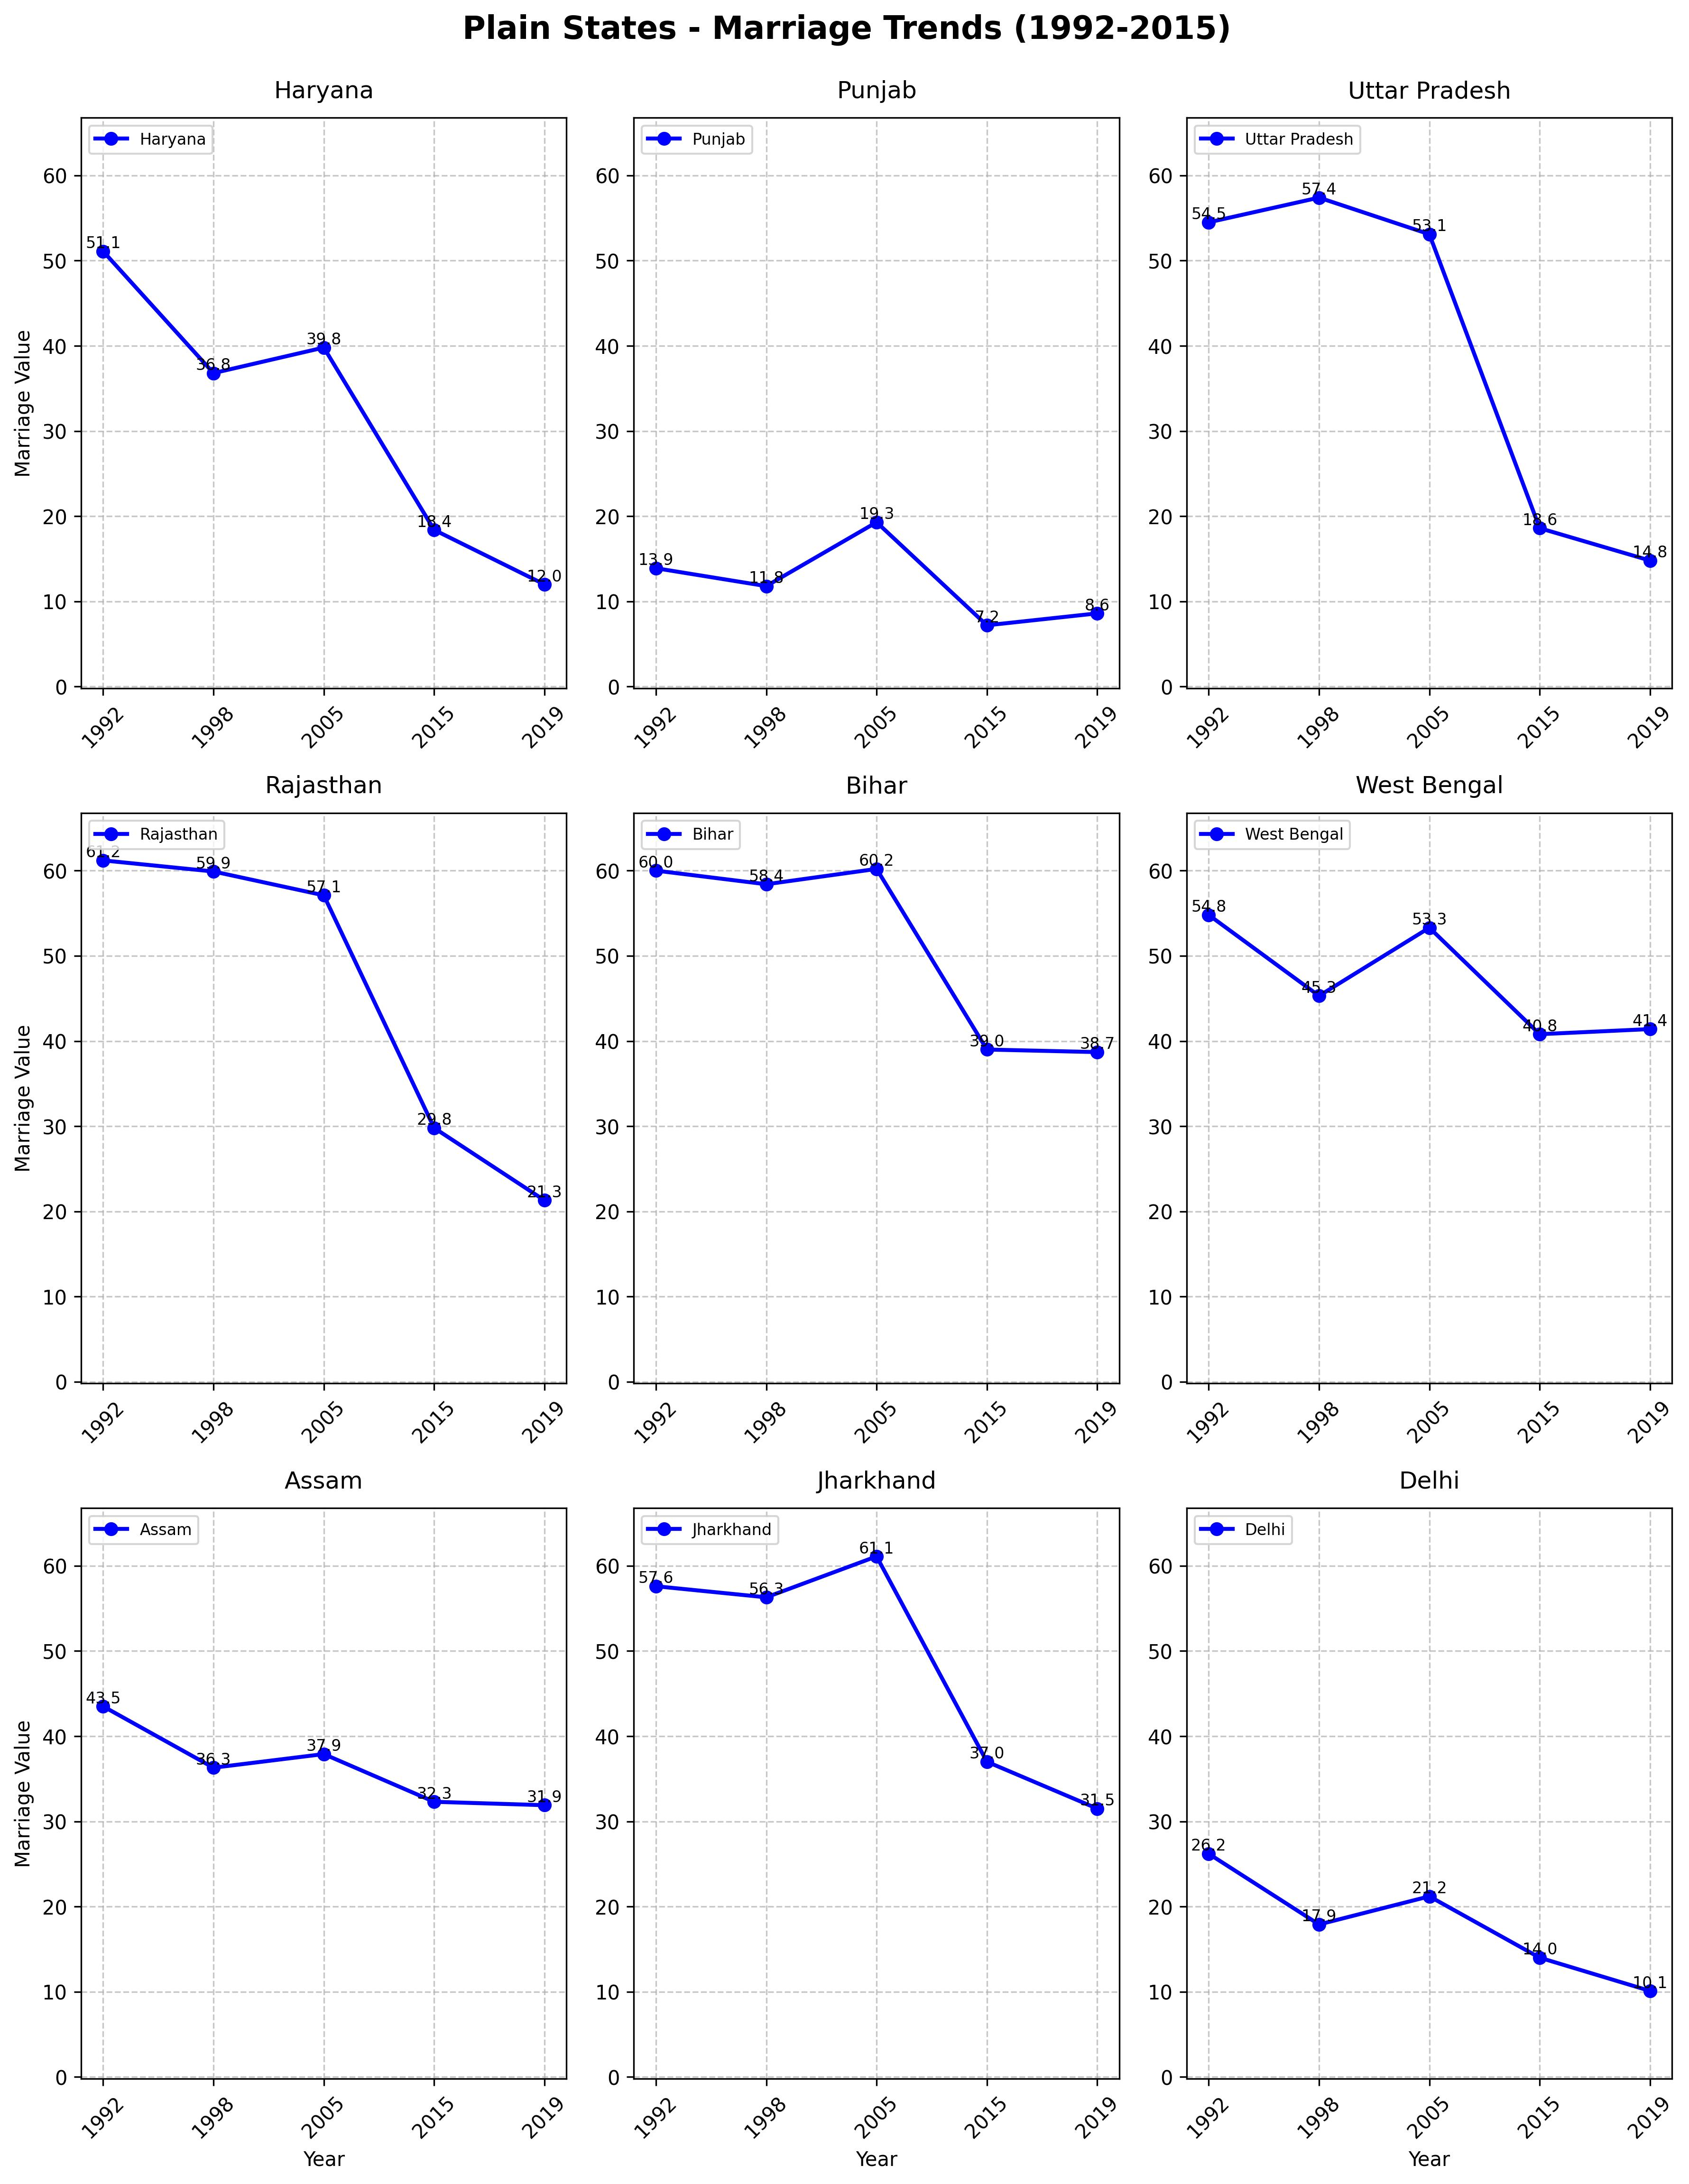
\includegraphics[width=0.9\textwidth, bb=0 0 800 800, clip]{figures/nfhs/plain_states_marriage_subplots.jpeg}
    \caption{Child Marriage age in Plain States}
    \label{fig:nfhs_plain_marriage}
\end{figure}

\begin{figure}[H]
    \centering
    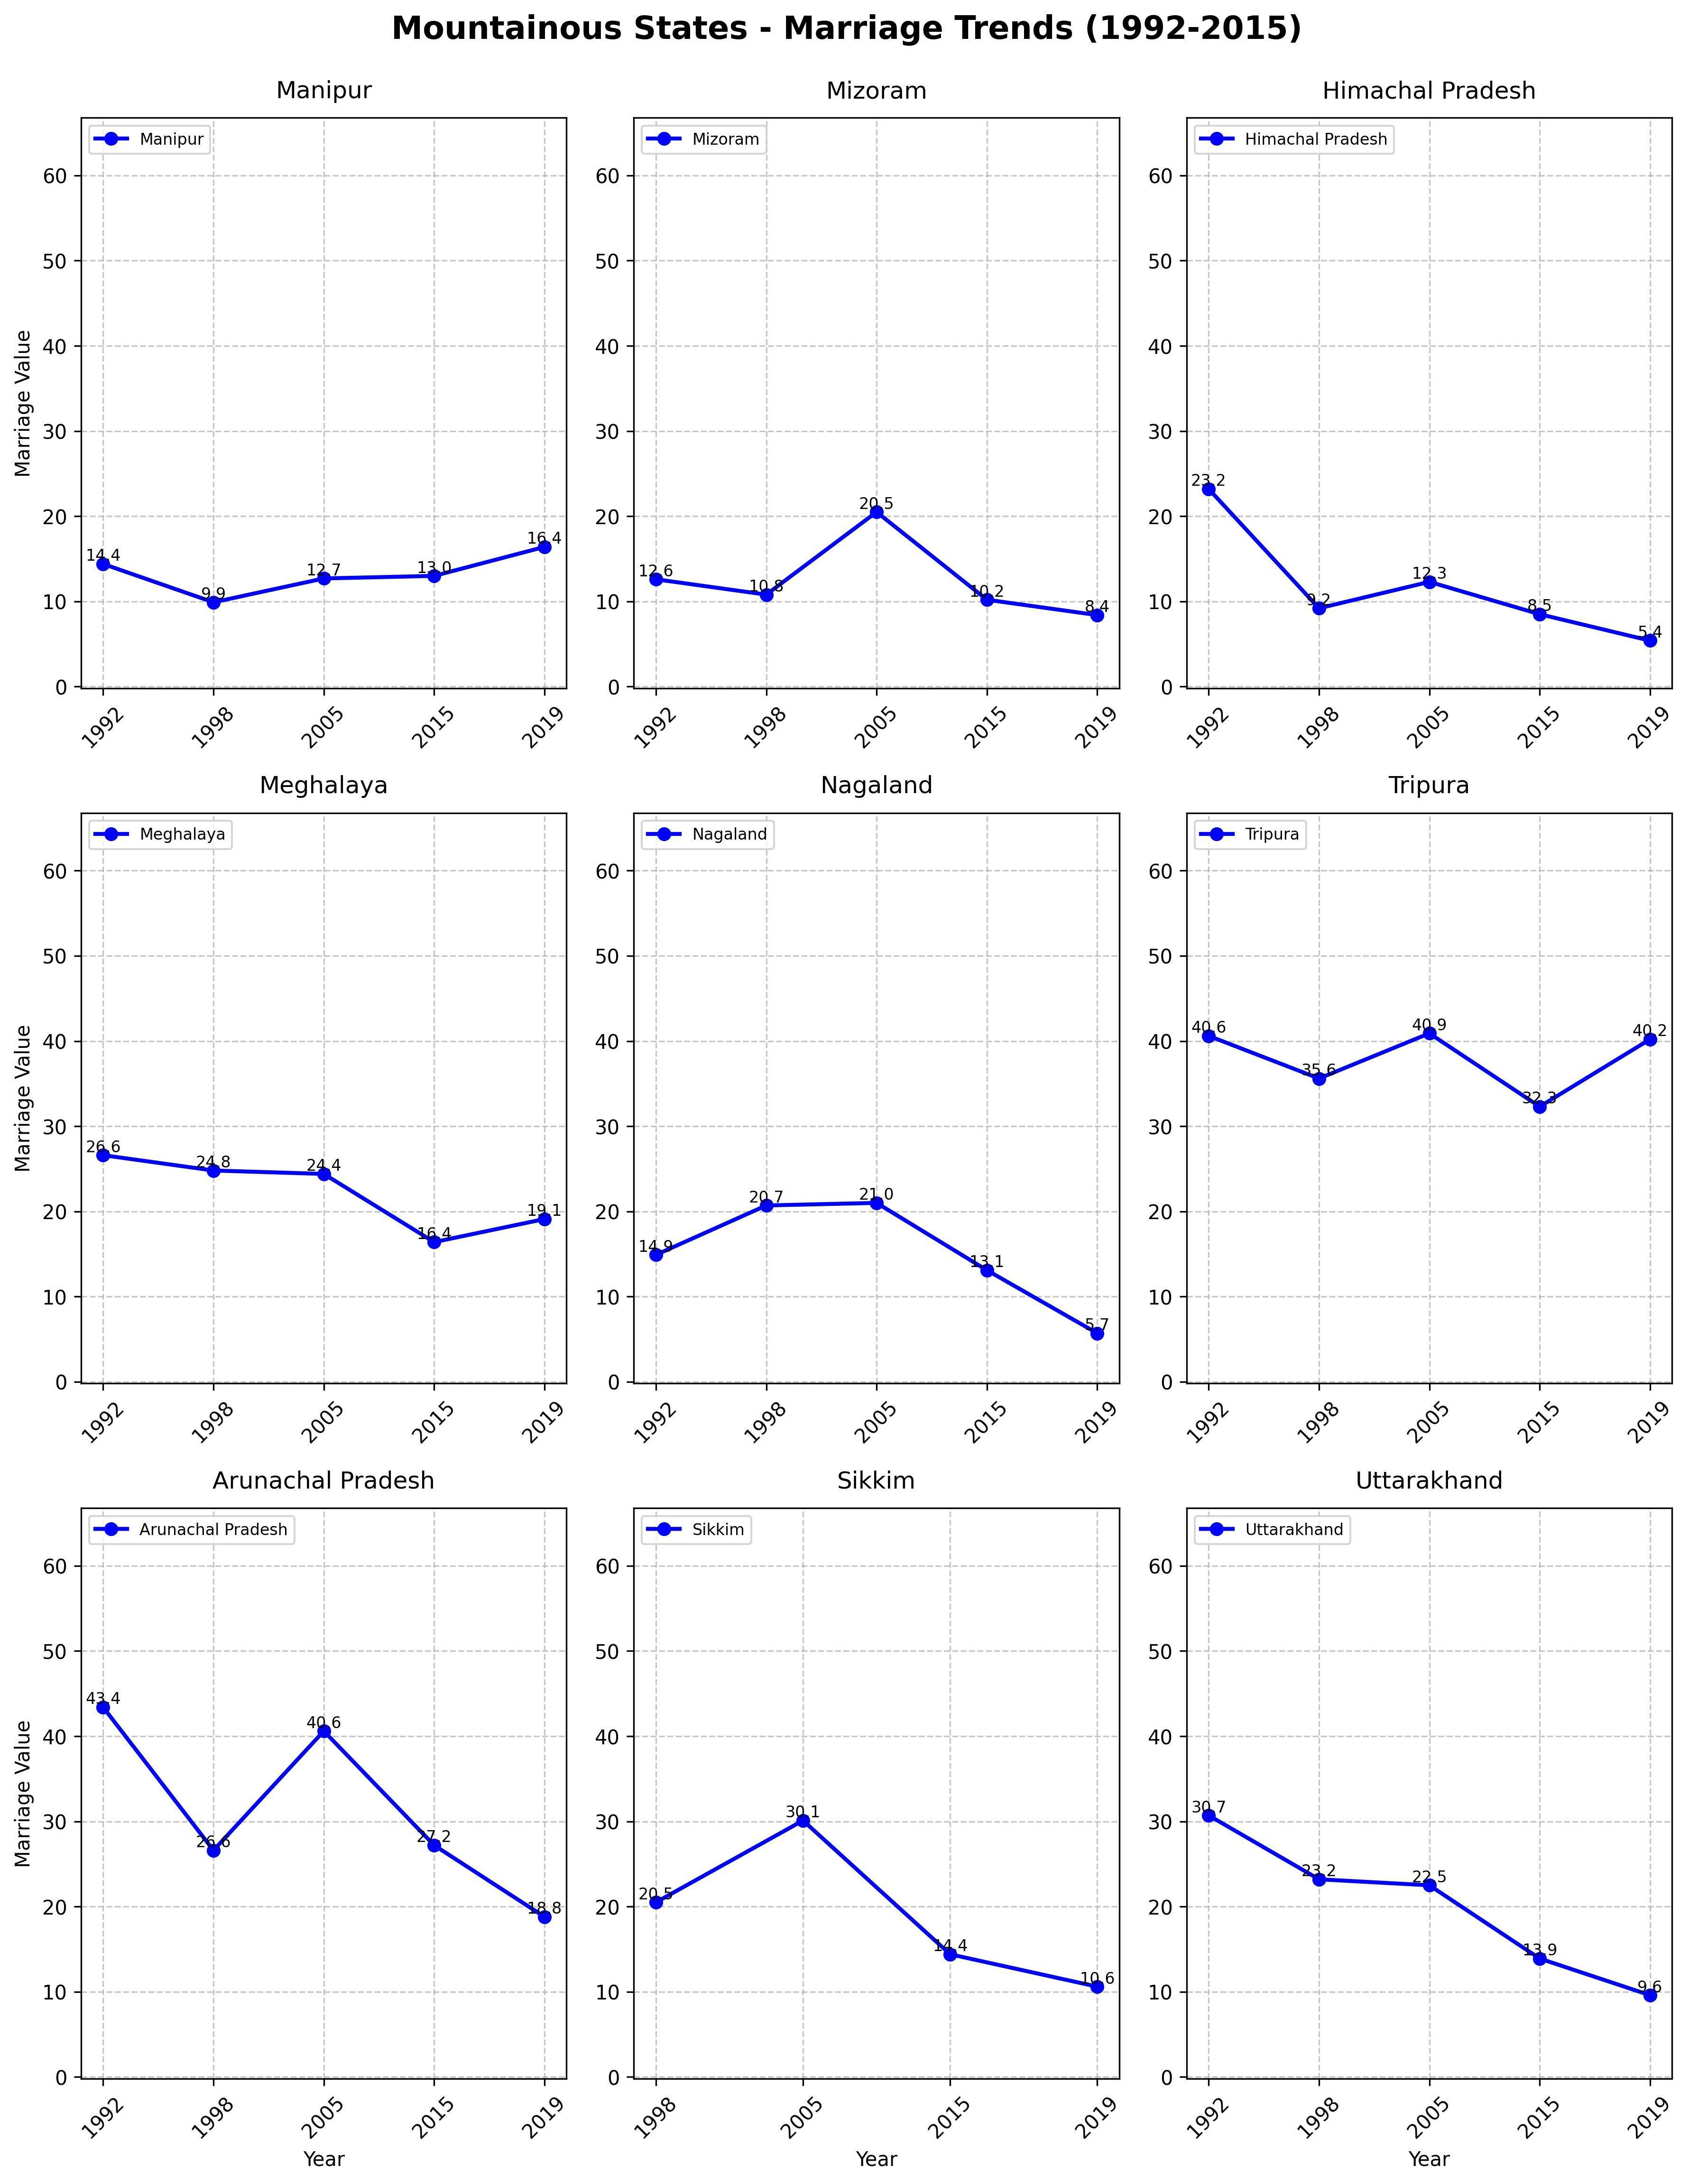
\includegraphics[width=0.9\textwidth, bb=0 0 800 800, clip]{figures/nfhs/mountainous_states_marriage_subplots.jpeg}
    \caption{Child Marriage age in Mountain States}
    \label{fig:nfhs_mountain_marriage}
\end{figure}
\end{document}
